% Created by tikzDevice version 0.12.6 on 2026-05-29 11:03:06
% !TEX encoding = UTF-8 Unicode
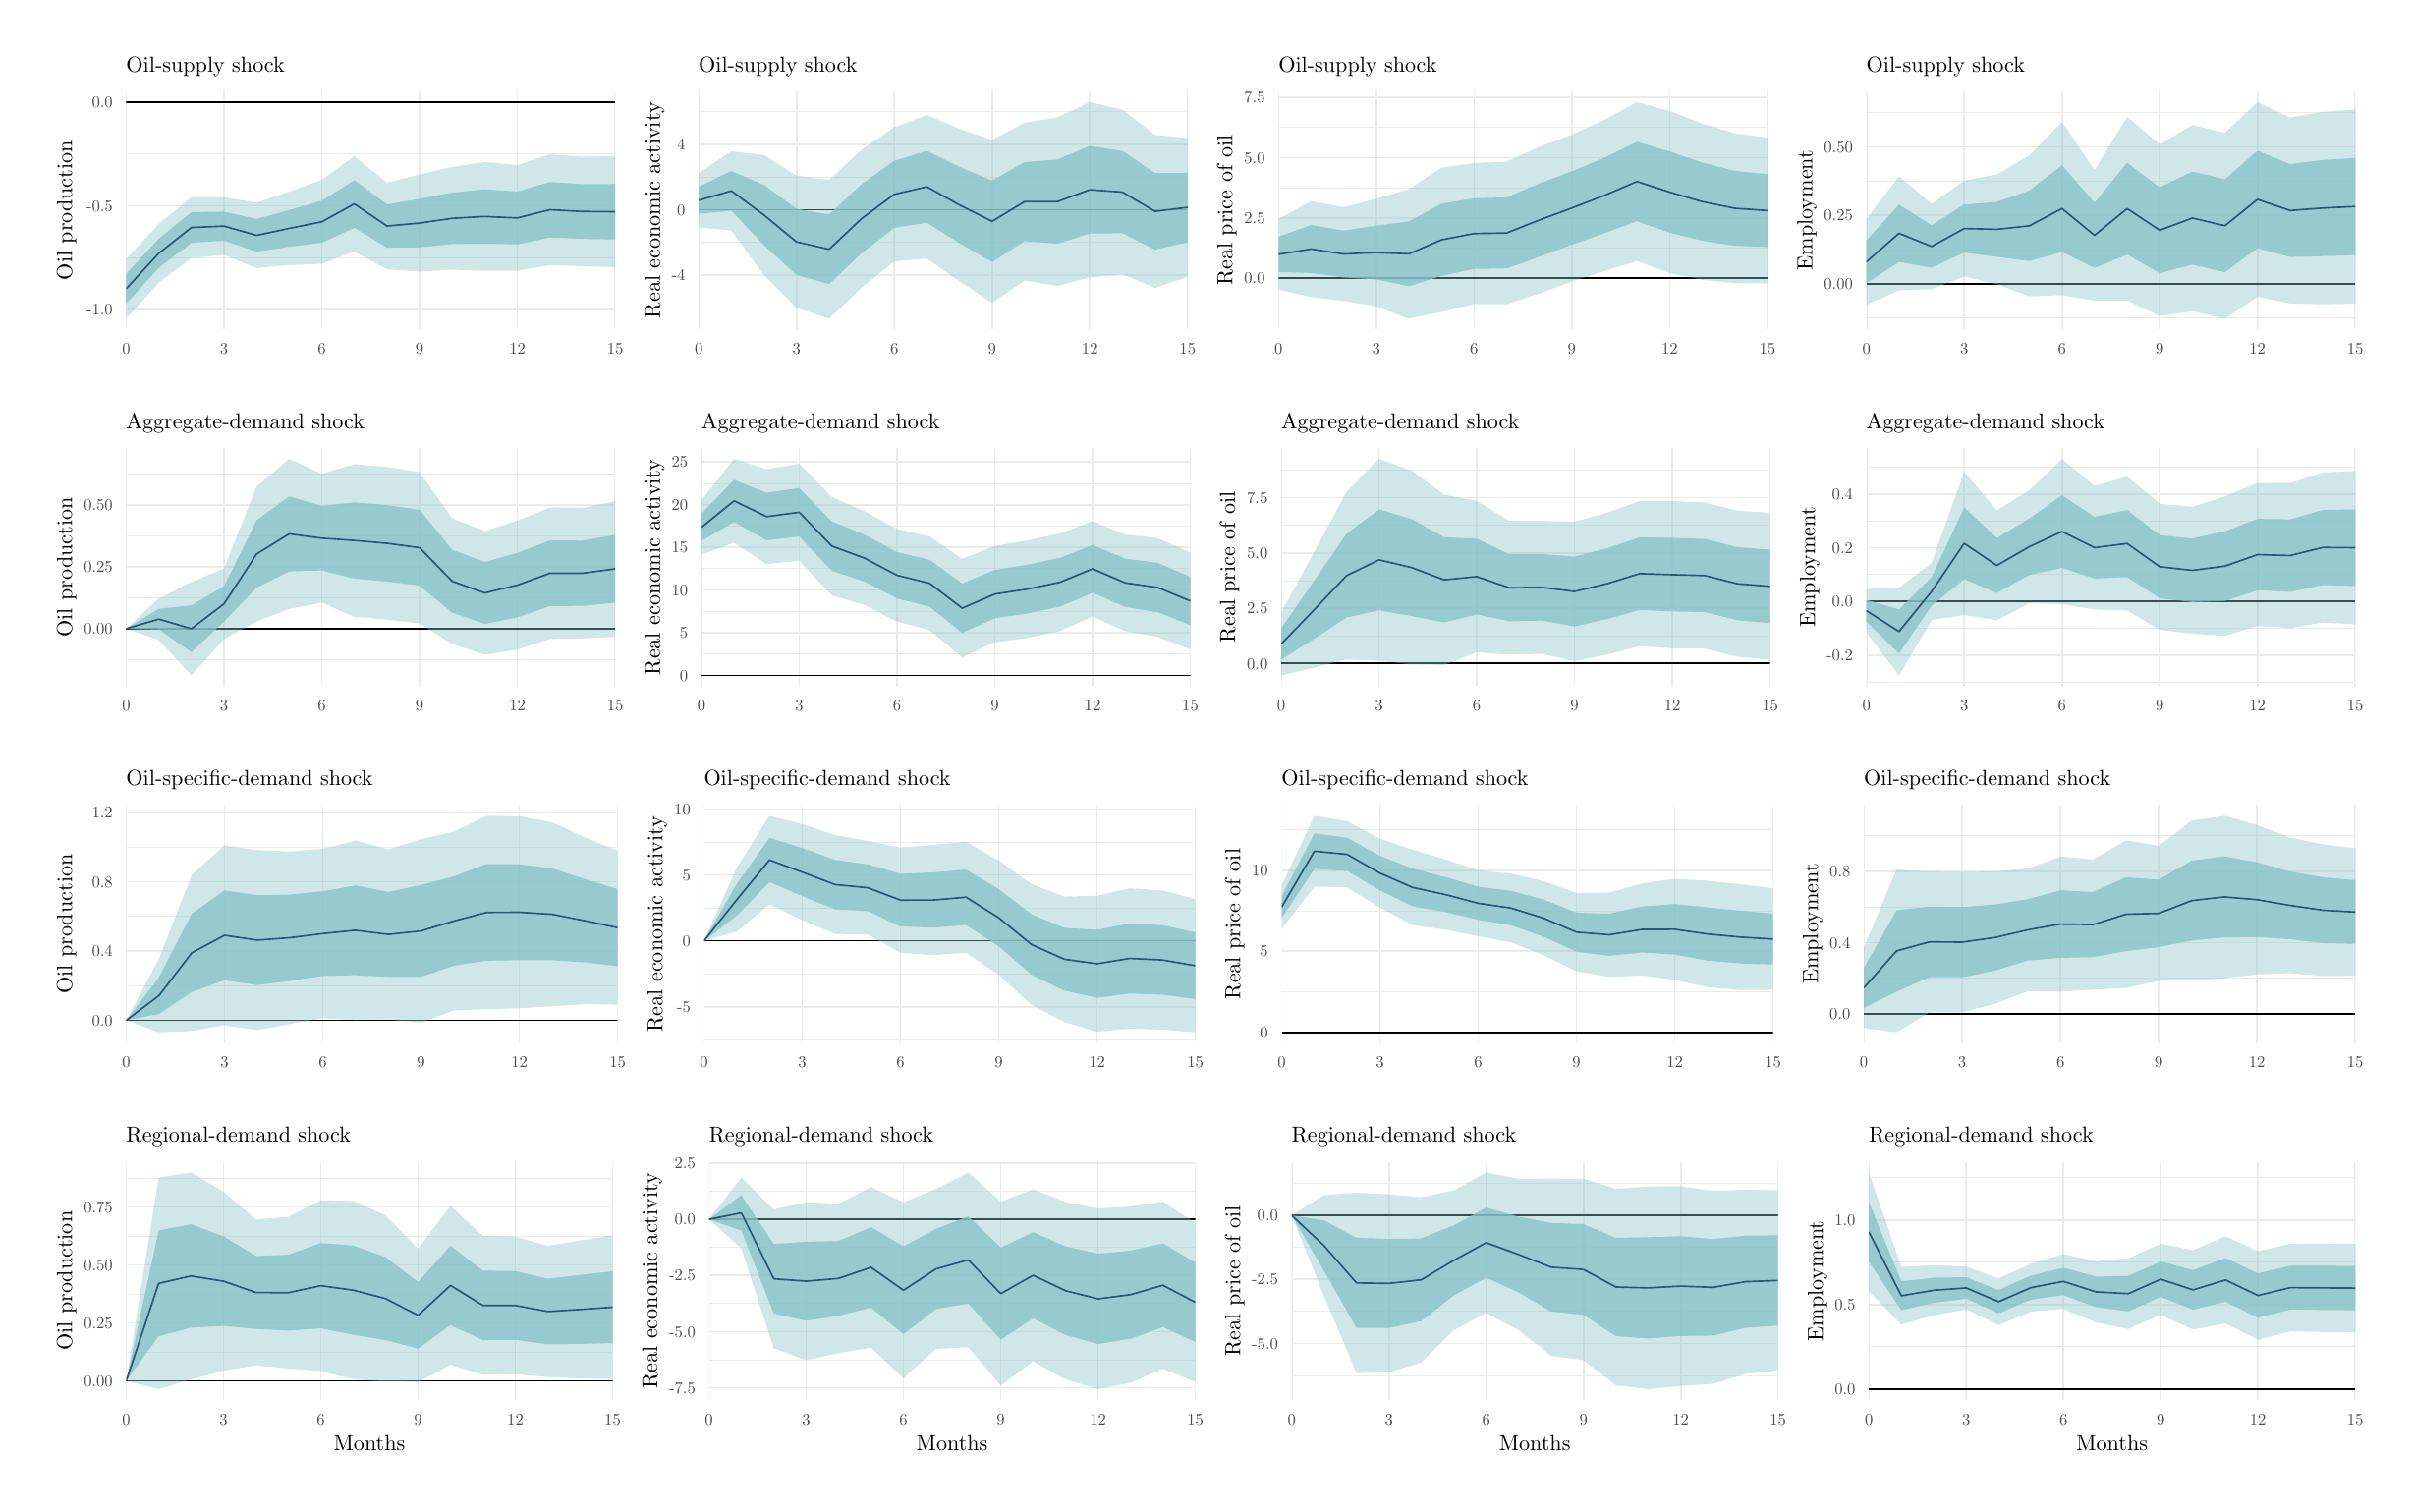
\begin{tikzpicture}[x=1pt,y=1pt]
\definecolor{fillColor}{RGB}{255,255,255}
\path[use as bounding box,fill=fillColor,fill opacity=0.00] (0,0) rectangle (867.24,535.98);
\begin{scope}
\path[clip] (  0.00,  0.00) rectangle (867.24,535.98);
\definecolor{drawColor}{RGB}{255,255,255}
\definecolor{fillColor}{RGB}{255,255,255}

\path[draw=drawColor,line width= 0.6pt,line join=round,line cap=round,fill=fillColor] (  0.00,  0.00) rectangle (867.24,535.98);
\end{scope}
\begin{scope}
\path[clip] (  5.50,399.24) rectangle (221.73,530.48);
\definecolor{fillColor}{RGB}{255,255,255}

\path[fill=fillColor] (  5.50,399.24) rectangle (221.73,530.48);
\end{scope}
\begin{scope}
\path[clip] (221.73,399.24) rectangle (432.29,530.48);
\definecolor{fillColor}{RGB}{255,255,255}

\path[fill=fillColor] (221.73,399.24) rectangle (432.29,530.48);
\end{scope}
\begin{scope}
\path[clip] (432.29,399.24) rectangle (645.51,530.48);
\definecolor{fillColor}{RGB}{255,255,255}

\path[fill=fillColor] (432.29,399.24) rectangle (645.51,530.48);
\end{scope}
\begin{scope}
\path[clip] (645.51,399.24) rectangle (861.74,530.48);
\definecolor{fillColor}{RGB}{255,255,255}

\path[fill=fillColor] (645.51,399.24) rectangle (861.74,530.48);
\end{scope}
\begin{scope}
\path[clip] ( 36.43,424.80) rectangle (216.23,512.42);
\definecolor{drawColor}{gray}{0.92}

\path[draw=drawColor,line width= 0.3pt,line join=round] ( 36.43,451.27) --
	(216.23,451.27);

\path[draw=drawColor,line width= 0.3pt,line join=round] ( 36.43,489.38) --
	(216.23,489.38);

\path[draw=drawColor,line width= 0.6pt,line join=round] ( 36.43,432.22) --
	(216.23,432.22);

\path[draw=drawColor,line width= 0.6pt,line join=round] ( 36.43,470.33) --
	(216.23,470.33);

\path[draw=drawColor,line width= 0.6pt,line join=round] ( 36.43,508.44) --
	(216.23,508.44);

\path[draw=drawColor,line width= 0.6pt,line join=round] ( 36.43,424.80) --
	( 36.43,512.42);

\path[draw=drawColor,line width= 0.6pt,line join=round] ( 72.39,424.80) --
	( 72.39,512.42);

\path[draw=drawColor,line width= 0.6pt,line join=round] (108.35,424.80) --
	(108.35,512.42);

\path[draw=drawColor,line width= 0.6pt,line join=round] (144.31,424.80) --
	(144.31,512.42);

\path[draw=drawColor,line width= 0.6pt,line join=round] (180.27,424.80) --
	(180.27,512.42);

\path[draw=drawColor,line width= 0.6pt,line join=round] (216.23,424.80) --
	(216.23,512.42);
\definecolor{drawColor}{RGB}{0,0,0}

\path[draw=drawColor,line width= 0.6pt,line join=round] ( 36.43,508.44) -- (216.23,508.44);
\definecolor{fillColor}{RGB}{136,195,200}

\path[fill=fillColor,fill opacity=0.40] ( 36.43,450.80) --
	( 48.42,463.55) --
	( 60.40,473.52) --
	( 72.39,473.44) --
	( 84.38,471.42) --
	( 96.36,475.44) --
	(108.35,479.86) --
	(120.33,488.51) --
	(132.32,478.75) --
	(144.31,481.76) --
	(156.29,484.57) --
	(168.28,486.33) --
	(180.27,485.27) --
	(192.25,489.22) --
	(204.24,488.33) --
	(216.23,488.52) --
	(216.23,447.73) --
	(204.24,448.04) --
	(192.25,448.45) --
	(180.27,446.36) --
	(168.28,446.37) --
	(156.29,446.76) --
	(144.31,446.08) --
	(132.32,446.94) --
	(120.33,453.42) --
	(108.35,448.95) --
	( 96.36,448.49) --
	( 84.38,447.39) --
	( 72.39,452.19) --
	( 60.40,451.06) --
	( 48.42,442.11) --
	( 36.43,428.78) --
	cycle;

\path[] ( 36.43,450.80) --
	( 48.42,463.55) --
	( 60.40,473.52) --
	( 72.39,473.44) --
	( 84.38,471.42) --
	( 96.36,475.44) --
	(108.35,479.86) --
	(120.33,488.51) --
	(132.32,478.75) --
	(144.31,481.76) --
	(156.29,484.57) --
	(168.28,486.33) --
	(180.27,485.27) --
	(192.25,489.22) --
	(204.24,488.33) --
	(216.23,488.52);

\path[] (216.23,447.73) --
	(204.24,448.04) --
	(192.25,448.45) --
	(180.27,446.36) --
	(168.28,446.37) --
	(156.29,446.76) --
	(144.31,446.08) --
	(132.32,446.94) --
	(120.33,453.42) --
	(108.35,448.95) --
	( 96.36,448.49) --
	( 84.38,447.39) --
	( 72.39,452.19) --
	( 60.40,451.06) --
	( 48.42,442.11) --
	( 36.43,428.78);
\definecolor{fillColor}{RGB}{136,195,200}

\path[fill=fillColor,fill opacity=0.80] ( 36.43,445.30) --
	( 48.42,458.19) --
	( 60.40,467.91) --
	( 72.39,468.13) --
	( 84.38,465.42) --
	( 96.36,468.70) --
	(108.35,472.13) --
	(120.33,479.74) --
	(132.32,470.80) --
	(144.31,472.84) --
	(156.29,475.12) --
	(168.28,476.34) --
	(180.27,475.54) --
	(192.25,479.03) --
	(204.24,478.26) --
	(216.23,478.32) --
	(216.23,457.93) --
	(204.24,458.11) --
	(192.25,458.64) --
	(180.27,456.08) --
	(168.28,456.36) --
	(156.29,456.21) --
	(144.31,455.00) --
	(132.32,454.89) --
	(120.33,462.20) --
	(108.35,456.67) --
	( 96.36,455.23) --
	( 84.38,453.40) --
	( 72.39,457.50) --
	( 60.40,456.67) --
	( 48.42,447.47) --
	( 36.43,434.29) --
	cycle;

\path[] ( 36.43,445.30) --
	( 48.42,458.19) --
	( 60.40,467.91) --
	( 72.39,468.13) --
	( 84.38,465.42) --
	( 96.36,468.70) --
	(108.35,472.13) --
	(120.33,479.74) --
	(132.32,470.80) --
	(144.31,472.84) --
	(156.29,475.12) --
	(168.28,476.34) --
	(180.27,475.54) --
	(192.25,479.03) --
	(204.24,478.26) --
	(216.23,478.32);

\path[] (216.23,457.93) --
	(204.24,458.11) --
	(192.25,458.64) --
	(180.27,456.08) --
	(168.28,456.36) --
	(156.29,456.21) --
	(144.31,455.00) --
	(132.32,454.89) --
	(120.33,462.20) --
	(108.35,456.67) --
	( 96.36,455.23) --
	( 84.38,453.40) --
	( 72.39,457.50) --
	( 60.40,456.67) --
	( 48.42,447.47) --
	( 36.43,434.29);
\definecolor{drawColor}{RGB}{42,86,118}

\path[draw=drawColor,line width= 0.6pt,line join=round] ( 36.43,439.79) --
	( 48.42,452.83) --
	( 60.40,462.29) --
	( 72.39,462.81) --
	( 84.38,459.41) --
	( 96.36,461.96) --
	(108.35,464.40) --
	(120.33,470.97) --
	(132.32,462.85) --
	(144.31,463.92) --
	(156.29,465.67) --
	(168.28,466.35) --
	(180.27,465.81) --
	(192.25,468.83) --
	(204.24,468.18) --
	(216.23,468.12);
\end{scope}
\begin{scope}
\path[clip] (  0.00,  0.00) rectangle (867.24,535.98);
\definecolor{drawColor}{gray}{0.30}

\node[text=drawColor,anchor=base east,inner sep=0pt, outer sep=0pt, scale=  0.60] at ( 31.48,430.15) {-1.0};

\node[text=drawColor,anchor=base east,inner sep=0pt, outer sep=0pt, scale=  0.60] at ( 31.48,468.26) {-0.5};

\node[text=drawColor,anchor=base east,inner sep=0pt, outer sep=0pt, scale=  0.60] at ( 31.48,506.37) {0.0};
\end{scope}
\begin{scope}
\path[clip] (  0.00,  0.00) rectangle (867.24,535.98);
\definecolor{drawColor}{gray}{0.30}

\node[text=drawColor,anchor=base,inner sep=0pt, outer sep=0pt, scale=  0.60] at ( 36.43,415.72) {0};

\node[text=drawColor,anchor=base,inner sep=0pt, outer sep=0pt, scale=  0.60] at ( 72.39,415.72) {3};

\node[text=drawColor,anchor=base,inner sep=0pt, outer sep=0pt, scale=  0.60] at (108.35,415.72) {6};

\node[text=drawColor,anchor=base,inner sep=0pt, outer sep=0pt, scale=  0.60] at (144.31,415.72) {9};

\node[text=drawColor,anchor=base,inner sep=0pt, outer sep=0pt, scale=  0.60] at (180.27,415.72) {12};

\node[text=drawColor,anchor=base,inner sep=0pt, outer sep=0pt, scale=  0.60] at (216.23,415.72) {15};
\end{scope}
\begin{scope}
\path[clip] (  0.00,  0.00) rectangle (867.24,535.98);
\definecolor{drawColor}{RGB}{0,0,0}

\node[text=drawColor,rotate= 90.00,anchor=base,inner sep=0pt, outer sep=0pt, scale=  0.80] at ( 16.51,468.61) {Oil production};
\end{scope}
\begin{scope}
\path[clip] (  0.00,  0.00) rectangle (867.24,535.98);
\definecolor{drawColor}{RGB}{0,0,0}

\node[text=drawColor,anchor=base west,inner sep=0pt, outer sep=0pt, scale=  0.80] at ( 36.43,519.47) {Oil-supply shock};
\end{scope}
\begin{scope}
\path[clip] (246.99,424.80) rectangle (426.79,512.42);
\definecolor{drawColor}{gray}{0.92}

\path[draw=drawColor,line width= 0.3pt,line join=round] (246.99,432.67) --
	(426.79,432.67);

\path[draw=drawColor,line width= 0.3pt,line join=round] (246.99,456.76) --
	(426.79,456.76);

\path[draw=drawColor,line width= 0.3pt,line join=round] (246.99,480.85) --
	(426.79,480.85);

\path[draw=drawColor,line width= 0.3pt,line join=round] (246.99,504.94) --
	(426.79,504.94);

\path[draw=drawColor,line width= 0.6pt,line join=round] (246.99,444.71) --
	(426.79,444.71);

\path[draw=drawColor,line width= 0.6pt,line join=round] (246.99,468.80) --
	(426.79,468.80);

\path[draw=drawColor,line width= 0.6pt,line join=round] (246.99,492.90) --
	(426.79,492.90);

\path[draw=drawColor,line width= 0.6pt,line join=round] (246.99,424.80) --
	(246.99,512.42);

\path[draw=drawColor,line width= 0.6pt,line join=round] (282.95,424.80) --
	(282.95,512.42);

\path[draw=drawColor,line width= 0.6pt,line join=round] (318.91,424.80) --
	(318.91,512.42);

\path[draw=drawColor,line width= 0.6pt,line join=round] (354.87,424.80) --
	(354.87,512.42);

\path[draw=drawColor,line width= 0.6pt,line join=round] (390.83,424.80) --
	(390.83,512.42);

\path[draw=drawColor,line width= 0.6pt,line join=round] (426.79,424.80) --
	(426.79,512.42);
\definecolor{drawColor}{RGB}{0,0,0}

\path[draw=drawColor,line width= 0.6pt,line join=round] (246.99,468.80) -- (426.79,468.80);
\definecolor{fillColor}{RGB}{136,195,200}

\path[fill=fillColor,fill opacity=0.40] (246.99,482.28) --
	(258.98,490.35) --
	(270.96,488.96) --
	(282.95,481.35) --
	(294.94,479.82) --
	(306.92,490.95) --
	(318.91,499.15) --
	(330.90,503.69) --
	(342.88,498.61) --
	(354.87,494.49) --
	(366.85,500.85) --
	(378.84,502.76) --
	(390.83,508.44) --
	(402.81,505.59) --
	(414.80,496.34) --
	(426.79,495.24) --
	(426.79,444.13) --
	(414.80,440.13) --
	(402.81,445.06) --
	(390.83,443.95) --
	(378.84,440.82) --
	(366.85,442.78) --
	(354.87,434.64) --
	(342.88,442.53) --
	(330.90,450.85) --
	(318.91,449.86) --
	(306.92,440.19) --
	(294.94,428.78) --
	(282.95,432.69) --
	(270.96,444.82) --
	(258.98,461.18) --
	(246.99,462.30) --
	cycle;

\path[] (246.99,482.28) --
	(258.98,490.35) --
	(270.96,488.96) --
	(282.95,481.35) --
	(294.94,479.82) --
	(306.92,490.95) --
	(318.91,499.15) --
	(330.90,503.69) --
	(342.88,498.61) --
	(354.87,494.49) --
	(366.85,500.85) --
	(378.84,502.76) --
	(390.83,508.44) --
	(402.81,505.59) --
	(414.80,496.34) --
	(426.79,495.24);

\path[] (426.79,444.13) --
	(414.80,440.13) --
	(402.81,445.06) --
	(390.83,443.95) --
	(378.84,440.82) --
	(366.85,442.78) --
	(354.87,434.64) --
	(342.88,442.53) --
	(330.90,450.85) --
	(318.91,449.86) --
	(306.92,440.19) --
	(294.94,428.78) --
	(282.95,432.69) --
	(270.96,444.82) --
	(258.98,461.18) --
	(246.99,462.30);
\definecolor{fillColor}{RGB}{136,195,200}

\path[fill=fillColor,fill opacity=0.80] (246.99,477.28) --
	(258.98,483.05) --
	(270.96,477.93) --
	(282.95,469.18) --
	(294.94,467.06) --
	(306.92,478.26) --
	(318.91,486.83) --
	(330.90,490.48) --
	(342.88,484.59) --
	(354.87,479.53) --
	(366.85,486.34) --
	(378.84,487.28) --
	(390.83,492.31) --
	(402.81,490.46) --
	(414.80,482.29) --
	(426.79,482.46) --
	(426.79,456.91) --
	(414.80,454.18) --
	(402.81,460.19) --
	(390.83,460.07) --
	(378.84,456.31) --
	(366.85,457.30) --
	(354.87,449.60) --
	(342.88,456.55) --
	(330.90,464.06) --
	(318.91,462.18) --
	(306.92,452.88) --
	(294.94,441.54) --
	(282.95,444.85) --
	(270.96,455.85) --
	(258.98,468.47) --
	(246.99,467.29) --
	cycle;

\path[] (246.99,477.28) --
	(258.98,483.05) --
	(270.96,477.93) --
	(282.95,469.18) --
	(294.94,467.06) --
	(306.92,478.26) --
	(318.91,486.83) --
	(330.90,490.48) --
	(342.88,484.59) --
	(354.87,479.53) --
	(366.85,486.34) --
	(378.84,487.28) --
	(390.83,492.31) --
	(402.81,490.46) --
	(414.80,482.29) --
	(426.79,482.46);

\path[] (426.79,456.91) --
	(414.80,454.18) --
	(402.81,460.19) --
	(390.83,460.07) --
	(378.84,456.31) --
	(366.85,457.30) --
	(354.87,449.60) --
	(342.88,456.55) --
	(330.90,464.06) --
	(318.91,462.18) --
	(306.92,452.88) --
	(294.94,441.54) --
	(282.95,444.85) --
	(270.96,455.85) --
	(258.98,468.47) --
	(246.99,467.29);
\definecolor{drawColor}{RGB}{42,86,118}

\path[draw=drawColor,line width= 0.6pt,line join=round] (246.99,472.29) --
	(258.98,475.76) --
	(270.96,466.89) --
	(282.95,457.02) --
	(294.94,454.30) --
	(306.92,465.57) --
	(318.91,474.51) --
	(330.90,477.27) --
	(342.88,470.57) --
	(354.87,464.56) --
	(366.85,471.82) --
	(378.84,471.79) --
	(390.83,476.19) --
	(402.81,475.32) --
	(414.80,468.24) --
	(426.79,469.69);
\end{scope}
\begin{scope}
\path[clip] (  0.00,  0.00) rectangle (867.24,535.98);
\definecolor{drawColor}{gray}{0.30}

\node[text=drawColor,anchor=base east,inner sep=0pt, outer sep=0pt, scale=  0.60] at (242.04,442.65) {-4};

\node[text=drawColor,anchor=base east,inner sep=0pt, outer sep=0pt, scale=  0.60] at (242.04,466.74) {0};

\node[text=drawColor,anchor=base east,inner sep=0pt, outer sep=0pt, scale=  0.60] at (242.04,490.83) {4};
\end{scope}
\begin{scope}
\path[clip] (  0.00,  0.00) rectangle (867.24,535.98);
\definecolor{drawColor}{gray}{0.30}

\node[text=drawColor,anchor=base,inner sep=0pt, outer sep=0pt, scale=  0.60] at (246.99,415.72) {0};

\node[text=drawColor,anchor=base,inner sep=0pt, outer sep=0pt, scale=  0.60] at (282.95,415.72) {3};

\node[text=drawColor,anchor=base,inner sep=0pt, outer sep=0pt, scale=  0.60] at (318.91,415.72) {6};

\node[text=drawColor,anchor=base,inner sep=0pt, outer sep=0pt, scale=  0.60] at (354.87,415.72) {9};

\node[text=drawColor,anchor=base,inner sep=0pt, outer sep=0pt, scale=  0.60] at (390.83,415.72) {12};

\node[text=drawColor,anchor=base,inner sep=0pt, outer sep=0pt, scale=  0.60] at (426.79,415.72) {15};
\end{scope}
\begin{scope}
\path[clip] (  0.00,  0.00) rectangle (867.24,535.98);
\definecolor{drawColor}{RGB}{0,0,0}

\node[text=drawColor,rotate= 90.00,anchor=base,inner sep=0pt, outer sep=0pt, scale=  0.80] at (232.74,468.61) {Real economic activity};
\end{scope}
\begin{scope}
\path[clip] (  0.00,  0.00) rectangle (867.24,535.98);
\definecolor{drawColor}{RGB}{0,0,0}

\node[text=drawColor,anchor=base west,inner sep=0pt, outer sep=0pt, scale=  0.80] at (246.99,519.47) {Oil-supply shock};
\end{scope}
\begin{scope}
\path[clip] (460.22,424.80) rectangle (640.01,512.42);
\definecolor{drawColor}{gray}{0.92}

\path[draw=drawColor,line width= 0.3pt,line join=round] (460.22,432.55) --
	(640.01,432.55);

\path[draw=drawColor,line width= 0.3pt,line join=round] (460.22,454.71) --
	(640.01,454.71);

\path[draw=drawColor,line width= 0.3pt,line join=round] (460.22,476.88) --
	(640.01,476.88);

\path[draw=drawColor,line width= 0.3pt,line join=round] (460.22,499.05) --
	(640.01,499.05);

\path[draw=drawColor,line width= 0.6pt,line join=round] (460.22,443.63) --
	(640.01,443.63);

\path[draw=drawColor,line width= 0.6pt,line join=round] (460.22,465.80) --
	(640.01,465.80);

\path[draw=drawColor,line width= 0.6pt,line join=round] (460.22,487.96) --
	(640.01,487.96);

\path[draw=drawColor,line width= 0.6pt,line join=round] (460.22,510.13) --
	(640.01,510.13);

\path[draw=drawColor,line width= 0.6pt,line join=round] (460.22,424.80) --
	(460.22,512.42);

\path[draw=drawColor,line width= 0.6pt,line join=round] (496.18,424.80) --
	(496.18,512.42);

\path[draw=drawColor,line width= 0.6pt,line join=round] (532.14,424.80) --
	(532.14,512.42);

\path[draw=drawColor,line width= 0.6pt,line join=round] (568.10,424.80) --
	(568.10,512.42);

\path[draw=drawColor,line width= 0.6pt,line join=round] (604.05,424.80) --
	(604.05,512.42);

\path[draw=drawColor,line width= 0.6pt,line join=round] (640.01,424.80) --
	(640.01,512.42);
\definecolor{drawColor}{RGB}{0,0,0}

\path[draw=drawColor,line width= 0.6pt,line join=round] (460.22,443.63) -- (640.01,443.63);
\definecolor{fillColor}{RGB}{136,195,200}

\path[fill=fillColor,fill opacity=0.40] (460.22,465.41) --
	(472.20,472.01) --
	(484.19,469.76) --
	(496.18,472.89) --
	(508.16,476.42) --
	(520.15,484.30) --
	(532.14,486.01) --
	(544.12,486.48) --
	(556.11,492.00) --
	(568.10,496.43) --
	(580.08,501.86) --
	(592.07,508.44) --
	(604.05,505.17) --
	(616.04,500.57) --
	(628.03,496.89) --
	(640.01,495.33) --
	(640.01,441.71) --
	(628.03,441.83) --
	(616.04,443.05) --
	(604.05,445.48) --
	(592.07,449.98) --
	(580.08,446.31) --
	(568.10,442.47) --
	(556.11,438.05) --
	(544.12,434.09) --
	(532.14,434.14) --
	(520.15,431.23) --
	(508.16,428.78) --
	(496.18,433.30) --
	(484.19,435.31) --
	(472.20,436.75) --
	(460.22,439.43) --
	cycle;

\path[] (460.22,465.41) --
	(472.20,472.01) --
	(484.19,469.76) --
	(496.18,472.89) --
	(508.16,476.42) --
	(520.15,484.30) --
	(532.14,486.01) --
	(544.12,486.48) --
	(556.11,492.00) --
	(568.10,496.43) --
	(580.08,501.86) --
	(592.07,508.44) --
	(604.05,505.17) --
	(616.04,500.57) --
	(628.03,496.89) --
	(640.01,495.33);

\path[] (640.01,441.71) --
	(628.03,441.83) --
	(616.04,443.05) --
	(604.05,445.48) --
	(592.07,449.98) --
	(580.08,446.31) --
	(568.10,442.47) --
	(556.11,438.05) --
	(544.12,434.09) --
	(532.14,434.14) --
	(520.15,431.23) --
	(508.16,428.78) --
	(496.18,433.30) --
	(484.19,435.31) --
	(472.20,436.75) --
	(460.22,439.43);
\definecolor{fillColor}{RGB}{136,195,200}

\path[fill=fillColor,fill opacity=0.80] (460.22,458.92) --
	(472.20,463.20) --
	(484.19,461.14) --
	(496.18,463.00) --
	(508.16,464.51) --
	(520.15,471.04) --
	(532.14,473.04) --
	(544.12,473.38) --
	(556.11,478.51) --
	(568.10,482.94) --
	(580.08,487.97) --
	(592.07,493.82) --
	(604.05,490.24) --
	(616.04,486.19) --
	(628.03,483.12) --
	(640.01,481.92) --
	(640.01,455.12) --
	(628.03,455.59) --
	(616.04,457.43) --
	(604.05,460.40) --
	(592.07,464.59) --
	(580.08,460.20) --
	(568.10,455.96) --
	(556.11,451.54) --
	(544.12,447.18) --
	(532.14,447.11) --
	(520.15,444.50) --
	(508.16,440.69) --
	(496.18,443.20) --
	(484.19,443.92) --
	(472.20,445.57) --
	(460.22,445.92) --
	cycle;

\path[] (460.22,458.92) --
	(472.20,463.20) --
	(484.19,461.14) --
	(496.18,463.00) --
	(508.16,464.51) --
	(520.15,471.04) --
	(532.14,473.04) --
	(544.12,473.38) --
	(556.11,478.51) --
	(568.10,482.94) --
	(580.08,487.97) --
	(592.07,493.82) --
	(604.05,490.24) --
	(616.04,486.19) --
	(628.03,483.12) --
	(640.01,481.92);

\path[] (640.01,455.12) --
	(628.03,455.59) --
	(616.04,457.43) --
	(604.05,460.40) --
	(592.07,464.59) --
	(580.08,460.20) --
	(568.10,455.96) --
	(556.11,451.54) --
	(544.12,447.18) --
	(532.14,447.11) --
	(520.15,444.50) --
	(508.16,440.69) --
	(496.18,443.20) --
	(484.19,443.92) --
	(472.20,445.57) --
	(460.22,445.92);
\definecolor{drawColor}{RGB}{42,86,118}

\path[draw=drawColor,line width= 0.6pt,line join=round] (460.22,452.42) --
	(472.20,454.38) --
	(484.19,452.53) --
	(496.18,453.10) --
	(508.16,452.60) --
	(520.15,457.77) --
	(532.14,460.07) --
	(544.12,460.28) --
	(556.11,465.03) --
	(568.10,469.45) --
	(580.08,474.09) --
	(592.07,479.21) --
	(604.05,475.32) --
	(616.04,471.81) --
	(628.03,469.36) --
	(640.01,468.52);
\end{scope}
\begin{scope}
\path[clip] (  0.00,  0.00) rectangle (867.24,535.98);
\definecolor{drawColor}{gray}{0.30}

\node[text=drawColor,anchor=base east,inner sep=0pt, outer sep=0pt, scale=  0.60] at (455.27,441.56) {0.0};

\node[text=drawColor,anchor=base east,inner sep=0pt, outer sep=0pt, scale=  0.60] at (455.27,463.73) {2.5};

\node[text=drawColor,anchor=base east,inner sep=0pt, outer sep=0pt, scale=  0.60] at (455.27,485.90) {5.0};

\node[text=drawColor,anchor=base east,inner sep=0pt, outer sep=0pt, scale=  0.60] at (455.27,508.07) {7.5};
\end{scope}
\begin{scope}
\path[clip] (  0.00,  0.00) rectangle (867.24,535.98);
\definecolor{drawColor}{gray}{0.30}

\node[text=drawColor,anchor=base,inner sep=0pt, outer sep=0pt, scale=  0.60] at (460.22,415.72) {0};

\node[text=drawColor,anchor=base,inner sep=0pt, outer sep=0pt, scale=  0.60] at (496.18,415.72) {3};

\node[text=drawColor,anchor=base,inner sep=0pt, outer sep=0pt, scale=  0.60] at (532.14,415.72) {6};

\node[text=drawColor,anchor=base,inner sep=0pt, outer sep=0pt, scale=  0.60] at (568.10,415.72) {9};

\node[text=drawColor,anchor=base,inner sep=0pt, outer sep=0pt, scale=  0.60] at (604.05,415.72) {12};

\node[text=drawColor,anchor=base,inner sep=0pt, outer sep=0pt, scale=  0.60] at (640.01,415.72) {15};
\end{scope}
\begin{scope}
\path[clip] (  0.00,  0.00) rectangle (867.24,535.98);
\definecolor{drawColor}{RGB}{0,0,0}

\node[text=drawColor,rotate= 90.00,anchor=base,inner sep=0pt, outer sep=0pt, scale=  0.80] at (443.30,468.61) {Real price of oil};
\end{scope}
\begin{scope}
\path[clip] (  0.00,  0.00) rectangle (867.24,535.98);
\definecolor{drawColor}{RGB}{0,0,0}

\node[text=drawColor,anchor=base west,inner sep=0pt, outer sep=0pt, scale=  0.80] at (460.22,519.47) {Oil-supply shock};
\end{scope}
\begin{scope}
\path[clip] (676.44,424.80) rectangle (856.24,512.42);
\definecolor{drawColor}{gray}{0.92}

\path[draw=drawColor,line width= 0.3pt,line join=round] (676.44,429.04) --
	(856.24,429.04);

\path[draw=drawColor,line width= 0.3pt,line join=round] (676.44,454.20) --
	(856.24,454.20);

\path[draw=drawColor,line width= 0.3pt,line join=round] (676.44,479.35) --
	(856.24,479.35);

\path[draw=drawColor,line width= 0.3pt,line join=round] (676.44,504.51) --
	(856.24,504.51);

\path[draw=drawColor,line width= 0.6pt,line join=round] (676.44,441.62) --
	(856.24,441.62);

\path[draw=drawColor,line width= 0.6pt,line join=round] (676.44,466.77) --
	(856.24,466.77);

\path[draw=drawColor,line width= 0.6pt,line join=round] (676.44,491.93) --
	(856.24,491.93);

\path[draw=drawColor,line width= 0.6pt,line join=round] (676.44,424.80) --
	(676.44,512.42);

\path[draw=drawColor,line width= 0.6pt,line join=round] (712.40,424.80) --
	(712.40,512.42);

\path[draw=drawColor,line width= 0.6pt,line join=round] (748.36,424.80) --
	(748.36,512.42);

\path[draw=drawColor,line width= 0.6pt,line join=round] (784.32,424.80) --
	(784.32,512.42);

\path[draw=drawColor,line width= 0.6pt,line join=round] (820.28,424.80) --
	(820.28,512.42);

\path[draw=drawColor,line width= 0.6pt,line join=round] (856.24,424.80) --
	(856.24,512.42);
\definecolor{drawColor}{RGB}{0,0,0}

\path[draw=drawColor,line width= 0.6pt,line join=round] (676.44,441.62) -- (856.24,441.62);
\definecolor{fillColor}{RGB}{136,195,200}

\path[fill=fillColor,fill opacity=0.40] (676.44,465.36) --
	(688.43,481.19) --
	(700.42,470.96) --
	(712.40,479.55) --
	(724.39,481.80) --
	(736.38,488.83) --
	(748.36,501.15) --
	(760.35,483.42) --
	(772.33,503.00) --
	(784.32,492.86) --
	(796.31,500.01) --
	(808.29,497.12) --
	(820.28,508.44) --
	(832.27,502.73) --
	(844.25,504.80) --
	(856.24,505.73) --
	(856.24,434.31) --
	(844.25,434.07) --
	(832.27,434.36) --
	(820.28,436.81) --
	(808.29,428.78) --
	(796.31,431.55) --
	(784.32,429.72) --
	(772.33,435.49) --
	(760.35,435.44) --
	(748.36,437.40) --
	(736.38,436.99) --
	(724.39,441.43) --
	(712.40,444.30) --
	(700.42,439.68) --
	(688.43,439.16) --
	(676.44,433.94) --
	cycle;

\path[] (676.44,465.36) --
	(688.43,481.19) --
	(700.42,470.96) --
	(712.40,479.55) --
	(724.39,481.80) --
	(736.38,488.83) --
	(748.36,501.15) --
	(760.35,483.42) --
	(772.33,503.00) --
	(784.32,492.86) --
	(796.31,500.01) --
	(808.29,497.12) --
	(820.28,508.44) --
	(832.27,502.73) --
	(844.25,504.80) --
	(856.24,505.73);

\path[] (856.24,434.31) --
	(844.25,434.07) --
	(832.27,434.36) --
	(820.28,436.81) --
	(808.29,428.78) --
	(796.31,431.55) --
	(784.32,429.72) --
	(772.33,435.49) --
	(760.35,435.44) --
	(748.36,437.40) --
	(736.38,436.99) --
	(724.39,441.43) --
	(712.40,444.30) --
	(700.42,439.68) --
	(688.43,439.16) --
	(676.44,433.94);
\definecolor{fillColor}{RGB}{136,195,200}

\path[fill=fillColor,fill opacity=0.80] (676.44,457.50) --
	(688.43,470.68) --
	(700.42,463.14) --
	(712.40,470.74) --
	(724.39,471.71) --
	(736.38,475.87) --
	(748.36,485.21) --
	(760.35,471.43) --
	(772.33,486.12) --
	(784.32,477.07) --
	(796.31,482.89) --
	(808.29,480.04) --
	(820.28,490.53) --
	(832.27,485.63) --
	(844.25,487.12) --
	(856.24,487.88) --
	(856.24,452.17) --
	(844.25,451.76) --
	(832.27,451.45) --
	(820.28,454.72) --
	(808.29,445.87) --
	(796.31,448.67) --
	(784.32,445.51) --
	(772.33,452.36) --
	(760.35,447.44) --
	(748.36,453.33) --
	(736.38,449.95) --
	(724.39,451.53) --
	(712.40,453.11) --
	(700.42,447.50) --
	(688.43,449.67) --
	(676.44,441.79) --
	cycle;

\path[] (676.44,457.50) --
	(688.43,470.68) --
	(700.42,463.14) --
	(712.40,470.74) --
	(724.39,471.71) --
	(736.38,475.87) --
	(748.36,485.21) --
	(760.35,471.43) --
	(772.33,486.12) --
	(784.32,477.07) --
	(796.31,482.89) --
	(808.29,480.04) --
	(820.28,490.53) --
	(832.27,485.63) --
	(844.25,487.12) --
	(856.24,487.88);

\path[] (856.24,452.17) --
	(844.25,451.76) --
	(832.27,451.45) --
	(820.28,454.72) --
	(808.29,445.87) --
	(796.31,448.67) --
	(784.32,445.51) --
	(772.33,452.36) --
	(760.35,447.44) --
	(748.36,453.33) --
	(736.38,449.95) --
	(724.39,451.53) --
	(712.40,453.11) --
	(700.42,447.50) --
	(688.43,449.67) --
	(676.44,441.79);
\definecolor{drawColor}{RGB}{42,86,118}

\path[draw=drawColor,line width= 0.6pt,line join=round] (676.44,449.65) --
	(688.43,460.17) --
	(700.42,455.32) --
	(712.40,461.93) --
	(724.39,461.62) --
	(736.38,462.91) --
	(748.36,469.27) --
	(760.35,459.43) --
	(772.33,469.24) --
	(784.32,461.29) --
	(796.31,465.78) --
	(808.29,462.95) --
	(820.28,472.62) --
	(832.27,468.54) --
	(844.25,469.44) --
	(856.24,470.02);
\end{scope}
\begin{scope}
\path[clip] (  0.00,  0.00) rectangle (867.24,535.98);
\definecolor{drawColor}{gray}{0.30}

\node[text=drawColor,anchor=base east,inner sep=0pt, outer sep=0pt, scale=  0.60] at (671.49,439.55) {0.00};

\node[text=drawColor,anchor=base east,inner sep=0pt, outer sep=0pt, scale=  0.60] at (671.49,464.71) {0.25};

\node[text=drawColor,anchor=base east,inner sep=0pt, outer sep=0pt, scale=  0.60] at (671.49,489.86) {0.50};
\end{scope}
\begin{scope}
\path[clip] (  0.00,  0.00) rectangle (867.24,535.98);
\definecolor{drawColor}{gray}{0.30}

\node[text=drawColor,anchor=base,inner sep=0pt, outer sep=0pt, scale=  0.60] at (676.44,415.72) {0};

\node[text=drawColor,anchor=base,inner sep=0pt, outer sep=0pt, scale=  0.60] at (712.40,415.72) {3};

\node[text=drawColor,anchor=base,inner sep=0pt, outer sep=0pt, scale=  0.60] at (748.36,415.72) {6};

\node[text=drawColor,anchor=base,inner sep=0pt, outer sep=0pt, scale=  0.60] at (784.32,415.72) {9};

\node[text=drawColor,anchor=base,inner sep=0pt, outer sep=0pt, scale=  0.60] at (820.28,415.72) {12};

\node[text=drawColor,anchor=base,inner sep=0pt, outer sep=0pt, scale=  0.60] at (856.24,415.72) {15};
\end{scope}
\begin{scope}
\path[clip] (  0.00,  0.00) rectangle (867.24,535.98);
\definecolor{drawColor}{RGB}{0,0,0}

\node[text=drawColor,rotate= 90.00,anchor=base,inner sep=0pt, outer sep=0pt, scale=  0.80] at (656.52,468.61) {Employment};
\end{scope}
\begin{scope}
\path[clip] (  0.00,  0.00) rectangle (867.24,535.98);
\definecolor{drawColor}{RGB}{0,0,0}

\node[text=drawColor,anchor=base west,inner sep=0pt, outer sep=0pt, scale=  0.80] at (676.44,519.47) {Oil-supply shock};
\end{scope}
\begin{scope}
\path[clip] (  5.50,267.99) rectangle (221.73,399.24);
\definecolor{fillColor}{RGB}{255,255,255}

\path[fill=fillColor] (  5.50,267.99) rectangle (221.73,399.24);
\end{scope}
\begin{scope}
\path[clip] (221.73,267.99) rectangle (433.29,399.24);
\definecolor{fillColor}{RGB}{255,255,255}

\path[fill=fillColor] (221.73,267.99) rectangle (433.29,399.24);
\end{scope}
\begin{scope}
\path[clip] (433.29,267.99) rectangle (646.51,399.24);
\definecolor{fillColor}{RGB}{255,255,255}

\path[fill=fillColor] (433.29,267.99) rectangle (646.51,399.24);
\end{scope}
\begin{scope}
\path[clip] (646.51,267.99) rectangle (861.74,399.24);
\definecolor{fillColor}{RGB}{255,255,255}

\path[fill=fillColor] (646.51,267.99) rectangle (861.74,399.24);
\end{scope}
\begin{scope}
\path[clip] ( 36.43,293.56) rectangle (216.23,381.17);
\definecolor{drawColor}{gray}{0.92}

\path[draw=drawColor,line width= 0.3pt,line join=round] ( 36.43,303.37) --
	(216.23,303.37);

\path[draw=drawColor,line width= 0.3pt,line join=round] ( 36.43,326.12) --
	(216.23,326.12);

\path[draw=drawColor,line width= 0.3pt,line join=round] ( 36.43,348.87) --
	(216.23,348.87);

\path[draw=drawColor,line width= 0.3pt,line join=round] ( 36.43,371.62) --
	(216.23,371.62);

\path[draw=drawColor,line width= 0.6pt,line join=round] ( 36.43,314.75) --
	(216.23,314.75);

\path[draw=drawColor,line width= 0.6pt,line join=round] ( 36.43,337.49) --
	(216.23,337.49);

\path[draw=drawColor,line width= 0.6pt,line join=round] ( 36.43,360.24) --
	(216.23,360.24);

\path[draw=drawColor,line width= 0.6pt,line join=round] ( 36.43,293.56) --
	( 36.43,381.17);

\path[draw=drawColor,line width= 0.6pt,line join=round] ( 72.39,293.56) --
	( 72.39,381.17);

\path[draw=drawColor,line width= 0.6pt,line join=round] (108.35,293.56) --
	(108.35,381.17);

\path[draw=drawColor,line width= 0.6pt,line join=round] (144.31,293.56) --
	(144.31,381.17);

\path[draw=drawColor,line width= 0.6pt,line join=round] (180.27,293.56) --
	(180.27,381.17);

\path[draw=drawColor,line width= 0.6pt,line join=round] (216.23,293.56) --
	(216.23,381.17);
\definecolor{drawColor}{RGB}{0,0,0}

\path[draw=drawColor,line width= 0.6pt,line join=round] ( 36.43,314.75) -- (216.23,314.75);
\definecolor{fillColor}{RGB}{136,195,200}

\path[fill=fillColor,fill opacity=0.40] ( 36.43,314.75) --
	( 48.42,325.87) --
	( 60.40,331.91) --
	( 72.39,336.82) --
	( 84.38,367.00) --
	( 96.36,377.19) --
	(108.35,371.74) --
	(120.33,375.22) --
	(132.32,374.21) --
	(144.31,372.33) --
	(156.29,355.29) --
	(168.28,350.63) --
	(180.27,354.46) --
	(192.25,359.29) --
	(204.24,359.12) --
	(216.23,361.72) --
	(216.23,311.78) --
	(204.24,311.15) --
	(192.25,310.97) --
	(180.27,307.05) --
	(168.28,305.15) --
	(156.29,309.11) --
	(144.31,316.72) --
	(132.32,318.06) --
	(120.33,319.13) --
	(108.35,324.30) --
	( 96.36,322.02) --
	( 84.38,317.41) --
	( 72.39,310.93) --
	( 60.40,297.54) --
	( 48.42,310.66) --
	( 36.43,314.75) --
	cycle;

\path[] ( 36.43,314.75) --
	( 48.42,325.87) --
	( 60.40,331.91) --
	( 72.39,336.82) --
	( 84.38,367.00) --
	( 96.36,377.19) --
	(108.35,371.74) --
	(120.33,375.22) --
	(132.32,374.21) --
	(144.31,372.33) --
	(156.29,355.29) --
	(168.28,350.63) --
	(180.27,354.46) --
	(192.25,359.29) --
	(204.24,359.12) --
	(216.23,361.72);

\path[] (216.23,311.78) --
	(204.24,311.15) --
	(192.25,310.97) --
	(180.27,307.05) --
	(168.28,305.15) --
	(156.29,309.11) --
	(144.31,316.72) --
	(132.32,318.06) --
	(120.33,319.13) --
	(108.35,324.30) --
	( 96.36,322.02) --
	( 84.38,317.41) --
	( 72.39,310.93) --
	( 60.40,297.54) --
	( 48.42,310.66) --
	( 36.43,314.75);
\definecolor{fillColor}{RGB}{136,195,200}

\path[fill=fillColor,fill opacity=0.80] ( 36.43,314.75) --
	( 48.42,322.06) --
	( 60.40,323.32) --
	( 72.39,330.35) --
	( 84.38,354.60) --
	( 96.36,363.40) --
	(108.35,359.88) --
	(120.33,361.20) --
	(132.32,360.18) --
	(144.31,358.43) --
	(156.29,343.75) --
	(168.28,339.26) --
	(180.27,342.61) --
	(192.25,347.21) --
	(204.24,347.13) --
	(216.23,349.23) --
	(216.23,324.27) --
	(204.24,323.14) --
	(192.25,323.05) --
	(180.27,318.90) --
	(168.28,316.52) --
	(156.29,320.66) --
	(144.31,330.62) --
	(132.32,332.10) --
	(120.33,333.15) --
	(108.35,336.16) --
	( 96.36,335.81) --
	( 84.38,329.81) --
	( 72.39,317.40) --
	( 60.40,306.13) --
	( 48.42,314.46) --
	( 36.43,314.75) --
	cycle;

\path[] ( 36.43,314.75) --
	( 48.42,322.06) --
	( 60.40,323.32) --
	( 72.39,330.35) --
	( 84.38,354.60) --
	( 96.36,363.40) --
	(108.35,359.88) --
	(120.33,361.20) --
	(132.32,360.18) --
	(144.31,358.43) --
	(156.29,343.75) --
	(168.28,339.26) --
	(180.27,342.61) --
	(192.25,347.21) --
	(204.24,347.13) --
	(216.23,349.23);

\path[] (216.23,324.27) --
	(204.24,323.14) --
	(192.25,323.05) --
	(180.27,318.90) --
	(168.28,316.52) --
	(156.29,320.66) --
	(144.31,330.62) --
	(132.32,332.10) --
	(120.33,333.15) --
	(108.35,336.16) --
	( 96.36,335.81) --
	( 84.38,329.81) --
	( 72.39,317.40) --
	( 60.40,306.13) --
	( 48.42,314.46) --
	( 36.43,314.75);
\definecolor{drawColor}{RGB}{42,86,118}

\path[draw=drawColor,line width= 0.6pt,line join=round] ( 36.43,314.75) --
	( 48.42,318.26) --
	( 60.40,314.72) --
	( 72.39,323.87) --
	( 84.38,342.20) --
	( 96.36,349.60) --
	(108.35,348.02) --
	(120.33,347.18) --
	(132.32,346.14) --
	(144.31,344.52) --
	(156.29,332.20) --
	(168.28,327.89) --
	(180.27,330.75) --
	(192.25,335.13) --
	(204.24,335.14) --
	(216.23,336.75);
\end{scope}
\begin{scope}
\path[clip] (  0.00,  0.00) rectangle (867.24,535.98);
\definecolor{drawColor}{gray}{0.30}

\node[text=drawColor,anchor=base east,inner sep=0pt, outer sep=0pt, scale=  0.60] at ( 31.48,312.68) {0.00};

\node[text=drawColor,anchor=base east,inner sep=0pt, outer sep=0pt, scale=  0.60] at ( 31.48,335.43) {0.25};

\node[text=drawColor,anchor=base east,inner sep=0pt, outer sep=0pt, scale=  0.60] at ( 31.48,358.18) {0.50};
\end{scope}
\begin{scope}
\path[clip] (  0.00,  0.00) rectangle (867.24,535.98);
\definecolor{drawColor}{gray}{0.30}

\node[text=drawColor,anchor=base,inner sep=0pt, outer sep=0pt, scale=  0.60] at ( 36.43,284.47) {0};

\node[text=drawColor,anchor=base,inner sep=0pt, outer sep=0pt, scale=  0.60] at ( 72.39,284.47) {3};

\node[text=drawColor,anchor=base,inner sep=0pt, outer sep=0pt, scale=  0.60] at (108.35,284.47) {6};

\node[text=drawColor,anchor=base,inner sep=0pt, outer sep=0pt, scale=  0.60] at (144.31,284.47) {9};

\node[text=drawColor,anchor=base,inner sep=0pt, outer sep=0pt, scale=  0.60] at (180.27,284.47) {12};

\node[text=drawColor,anchor=base,inner sep=0pt, outer sep=0pt, scale=  0.60] at (216.23,284.47) {15};
\end{scope}
\begin{scope}
\path[clip] (  0.00,  0.00) rectangle (867.24,535.98);
\definecolor{drawColor}{RGB}{0,0,0}

\node[text=drawColor,rotate= 90.00,anchor=base,inner sep=0pt, outer sep=0pt, scale=  0.80] at ( 16.51,337.36) {Oil production};
\end{scope}
\begin{scope}
\path[clip] (  0.00,  0.00) rectangle (867.24,535.98);
\definecolor{drawColor}{RGB}{0,0,0}

\node[text=drawColor,anchor=base west,inner sep=0pt, outer sep=0pt, scale=  0.80] at ( 36.43,388.23) {Aggregate-demand shock};
\end{scope}
\begin{scope}
\path[clip] (247.99,293.56) rectangle (427.79,381.17);
\definecolor{drawColor}{gray}{0.92}

\path[draw=drawColor,line width= 0.3pt,line join=round] (247.99,305.39) --
	(427.79,305.39);

\path[draw=drawColor,line width= 0.3pt,line join=round] (247.99,321.09) --
	(427.79,321.09);

\path[draw=drawColor,line width= 0.3pt,line join=round] (247.99,336.79) --
	(427.79,336.79);

\path[draw=drawColor,line width= 0.3pt,line join=round] (247.99,352.49) --
	(427.79,352.49);

\path[draw=drawColor,line width= 0.3pt,line join=round] (247.99,368.19) --
	(427.79,368.19);

\path[draw=drawColor,line width= 0.6pt,line join=round] (247.99,297.54) --
	(427.79,297.54);

\path[draw=drawColor,line width= 0.6pt,line join=round] (247.99,313.24) --
	(427.79,313.24);

\path[draw=drawColor,line width= 0.6pt,line join=round] (247.99,328.94) --
	(427.79,328.94);

\path[draw=drawColor,line width= 0.6pt,line join=round] (247.99,344.64) --
	(427.79,344.64);

\path[draw=drawColor,line width= 0.6pt,line join=round] (247.99,360.34) --
	(427.79,360.34);

\path[draw=drawColor,line width= 0.6pt,line join=round] (247.99,376.04) --
	(427.79,376.04);

\path[draw=drawColor,line width= 0.6pt,line join=round] (247.99,293.56) --
	(247.99,381.17);

\path[draw=drawColor,line width= 0.6pt,line join=round] (283.95,293.56) --
	(283.95,381.17);

\path[draw=drawColor,line width= 0.6pt,line join=round] (319.91,293.56) --
	(319.91,381.17);

\path[draw=drawColor,line width= 0.6pt,line join=round] (355.87,293.56) --
	(355.87,381.17);

\path[draw=drawColor,line width= 0.6pt,line join=round] (391.83,293.56) --
	(391.83,381.17);

\path[draw=drawColor,line width= 0.6pt,line join=round] (427.79,293.56) --
	(427.79,381.17);
\definecolor{drawColor}{RGB}{0,0,0}

\path[draw=drawColor,line width= 0.6pt,line join=round] (247.99,297.54) -- (427.79,297.54);
\definecolor{fillColor}{RGB}{136,195,200}

\path[fill=fillColor,fill opacity=0.40] (247.99,362.02) --
	(259.98,377.19) --
	(271.96,373.42) --
	(283.95,375.40) --
	(295.94,363.22) --
	(307.92,357.91) --
	(319.91,351.42) --
	(331.89,348.68) --
	(343.88,340.39) --
	(355.87,345.18) --
	(367.85,347.25) --
	(379.84,349.76) --
	(391.83,354.26) --
	(403.81,349.36) --
	(415.80,348.03) --
	(427.79,342.71) --
	(427.79,307.16) --
	(415.80,311.75) --
	(403.81,313.86) --
	(391.83,319.23) --
	(379.84,313.88) --
	(367.85,311.35) --
	(355.87,309.75) --
	(343.88,304.17) --
	(331.89,314.22) --
	(319.91,317.34) --
	(307.92,323.51) --
	(295.94,326.99) --
	(283.95,339.71) --
	(271.96,338.51) --
	(259.98,346.32) --
	(247.99,342.03) --
	cycle;

\path[] (247.99,362.02) --
	(259.98,377.19) --
	(271.96,373.42) --
	(283.95,375.40) --
	(295.94,363.22) --
	(307.92,357.91) --
	(319.91,351.42) --
	(331.89,348.68) --
	(343.88,340.39) --
	(355.87,345.18) --
	(367.85,347.25) --
	(379.84,349.76) --
	(391.83,354.26) --
	(403.81,349.36) --
	(415.80,348.03) --
	(427.79,342.71);

\path[] (427.79,307.16) --
	(415.80,311.75) --
	(403.81,313.86) --
	(391.83,319.23) --
	(379.84,313.88) --
	(367.85,311.35) --
	(355.87,309.75) --
	(343.88,304.17) --
	(331.89,314.22) --
	(319.91,317.34) --
	(307.92,323.51) --
	(295.94,326.99) --
	(283.95,339.71) --
	(271.96,338.51) --
	(259.98,346.32) --
	(247.99,342.03);
\definecolor{fillColor}{RGB}{136,195,200}

\path[fill=fillColor,fill opacity=0.80] (247.99,357.02) --
	(259.98,369.47) --
	(271.96,364.69) --
	(283.95,366.48) --
	(295.94,354.17) --
	(307.92,349.31) --
	(319.91,342.90) --
	(331.89,340.06) --
	(343.88,331.34) --
	(355.87,336.32) --
	(367.85,338.27) --
	(379.84,340.79) --
	(391.83,345.50) --
	(403.81,340.49) --
	(415.80,338.96) --
	(427.79,333.82) --
	(427.79,316.05) --
	(415.80,320.82) --
	(403.81,322.74) --
	(391.83,327.99) --
	(379.84,322.85) --
	(367.85,320.32) --
	(355.87,318.61) --
	(343.88,313.23) --
	(331.89,322.83) --
	(319.91,325.86) --
	(307.92,332.11) --
	(295.94,336.05) --
	(283.95,348.63) --
	(271.96,347.24) --
	(259.98,354.03) --
	(247.99,347.03) --
	cycle;

\path[] (247.99,357.02) --
	(259.98,369.47) --
	(271.96,364.69) --
	(283.95,366.48) --
	(295.94,354.17) --
	(307.92,349.31) --
	(319.91,342.90) --
	(331.89,340.06) --
	(343.88,331.34) --
	(355.87,336.32) --
	(367.85,338.27) --
	(379.84,340.79) --
	(391.83,345.50) --
	(403.81,340.49) --
	(415.80,338.96) --
	(427.79,333.82);

\path[] (427.79,316.05) --
	(415.80,320.82) --
	(403.81,322.74) --
	(391.83,327.99) --
	(379.84,322.85) --
	(367.85,320.32) --
	(355.87,318.61) --
	(343.88,313.23) --
	(331.89,322.83) --
	(319.91,325.86) --
	(307.92,332.11) --
	(295.94,336.05) --
	(283.95,348.63) --
	(271.96,347.24) --
	(259.98,354.03) --
	(247.99,347.03);
\definecolor{drawColor}{RGB}{42,86,118}

\path[draw=drawColor,line width= 0.6pt,line join=round] (247.99,352.02) --
	(259.98,361.75) --
	(271.96,355.97) --
	(283.95,357.55) --
	(295.94,345.11) --
	(307.92,340.71) --
	(319.91,334.38) --
	(331.89,331.45) --
	(343.88,322.28) --
	(355.87,327.46) --
	(367.85,329.30) --
	(379.84,331.82) --
	(391.83,336.75) --
	(403.81,331.61) --
	(415.80,329.89) --
	(427.79,324.94);
\end{scope}
\begin{scope}
\path[clip] (  0.00,  0.00) rectangle (867.24,535.98);
\definecolor{drawColor}{gray}{0.30}

\node[text=drawColor,anchor=base east,inner sep=0pt, outer sep=0pt, scale=  0.60] at (243.04,295.47) {0};

\node[text=drawColor,anchor=base east,inner sep=0pt, outer sep=0pt, scale=  0.60] at (243.04,311.17) {5};

\node[text=drawColor,anchor=base east,inner sep=0pt, outer sep=0pt, scale=  0.60] at (243.04,326.87) {10};

\node[text=drawColor,anchor=base east,inner sep=0pt, outer sep=0pt, scale=  0.60] at (243.04,342.57) {15};

\node[text=drawColor,anchor=base east,inner sep=0pt, outer sep=0pt, scale=  0.60] at (243.04,358.28) {20};

\node[text=drawColor,anchor=base east,inner sep=0pt, outer sep=0pt, scale=  0.60] at (243.04,373.98) {25};
\end{scope}
\begin{scope}
\path[clip] (  0.00,  0.00) rectangle (867.24,535.98);
\definecolor{drawColor}{gray}{0.30}

\node[text=drawColor,anchor=base,inner sep=0pt, outer sep=0pt, scale=  0.60] at (247.99,284.47) {0};

\node[text=drawColor,anchor=base,inner sep=0pt, outer sep=0pt, scale=  0.60] at (283.95,284.47) {3};

\node[text=drawColor,anchor=base,inner sep=0pt, outer sep=0pt, scale=  0.60] at (319.91,284.47) {6};

\node[text=drawColor,anchor=base,inner sep=0pt, outer sep=0pt, scale=  0.60] at (355.87,284.47) {9};

\node[text=drawColor,anchor=base,inner sep=0pt, outer sep=0pt, scale=  0.60] at (391.83,284.47) {12};

\node[text=drawColor,anchor=base,inner sep=0pt, outer sep=0pt, scale=  0.60] at (427.79,284.47) {15};
\end{scope}
\begin{scope}
\path[clip] (  0.00,  0.00) rectangle (867.24,535.98);
\definecolor{drawColor}{RGB}{0,0,0}

\node[text=drawColor,rotate= 90.00,anchor=base,inner sep=0pt, outer sep=0pt, scale=  0.80] at (232.74,337.36) {Real economic activity};
\end{scope}
\begin{scope}
\path[clip] (  0.00,  0.00) rectangle (867.24,535.98);
\definecolor{drawColor}{RGB}{0,0,0}

\node[text=drawColor,anchor=base west,inner sep=0pt, outer sep=0pt, scale=  0.80] at (247.99,388.23) {Aggregate-demand shock};
\end{scope}
\begin{scope}
\path[clip] (461.22,293.56) rectangle (641.01,381.17);
\definecolor{drawColor}{gray}{0.92}

\path[draw=drawColor,line width= 0.3pt,line join=round] (461.22,312.12) --
	(641.01,312.12);

\path[draw=drawColor,line width= 0.3pt,line join=round] (461.22,332.44) --
	(641.01,332.44);

\path[draw=drawColor,line width= 0.3pt,line join=round] (461.22,352.76) --
	(641.01,352.76);

\path[draw=drawColor,line width= 0.3pt,line join=round] (461.22,373.07) --
	(641.01,373.07);

\path[draw=drawColor,line width= 0.6pt,line join=round] (461.22,301.96) --
	(641.01,301.96);

\path[draw=drawColor,line width= 0.6pt,line join=round] (461.22,322.28) --
	(641.01,322.28);

\path[draw=drawColor,line width= 0.6pt,line join=round] (461.22,342.60) --
	(641.01,342.60);

\path[draw=drawColor,line width= 0.6pt,line join=round] (461.22,362.92) --
	(641.01,362.92);

\path[draw=drawColor,line width= 0.6pt,line join=round] (461.22,293.56) --
	(461.22,381.17);

\path[draw=drawColor,line width= 0.6pt,line join=round] (497.18,293.56) --
	(497.18,381.17);

\path[draw=drawColor,line width= 0.6pt,line join=round] (533.14,293.56) --
	(533.14,381.17);

\path[draw=drawColor,line width= 0.6pt,line join=round] (569.09,293.56) --
	(569.09,381.17);

\path[draw=drawColor,line width= 0.6pt,line join=round] (605.05,293.56) --
	(605.05,381.17);

\path[draw=drawColor,line width= 0.6pt,line join=round] (641.01,293.56) --
	(641.01,381.17);
\definecolor{drawColor}{RGB}{0,0,0}

\path[draw=drawColor,line width= 0.6pt,line join=round] (461.22,301.96) -- (641.01,301.96);
\definecolor{fillColor}{RGB}{136,195,200}

\path[fill=fillColor,fill opacity=0.40] (461.22,320.71) --
	(473.20,342.71) --
	(485.19,364.99) --
	(497.18,377.19) --
	(509.16,372.88) --
	(521.15,364.04) --
	(533.14,361.72) --
	(545.12,354.39) --
	(557.11,354.42) --
	(569.09,354.06) --
	(581.08,357.39) --
	(593.07,361.65) --
	(605.05,361.66) --
	(617.04,361.19) --
	(629.03,358.12) --
	(641.01,357.36) --
	(641.01,303.30) --
	(629.03,304.41) --
	(617.04,307.40) --
	(605.05,307.54) --
	(593.07,308.32) --
	(581.08,305.23) --
	(569.09,302.76) --
	(557.11,305.49) --
	(545.12,305.18) --
	(533.14,306.09) --
	(521.15,301.37) --
	(509.16,301.57) --
	(497.18,302.93) --
	(485.19,303.45) --
	(473.20,300.38) --
	(461.22,297.54) --
	cycle;

\path[] (461.22,320.71) --
	(473.20,342.71) --
	(485.19,364.99) --
	(497.18,377.19) --
	(509.16,372.88) --
	(521.15,364.04) --
	(533.14,361.72) --
	(545.12,354.39) --
	(557.11,354.42) --
	(569.09,354.06) --
	(581.08,357.39) --
	(593.07,361.65) --
	(605.05,361.66) --
	(617.04,361.19) --
	(629.03,358.12) --
	(641.01,357.36);

\path[] (641.01,303.30) --
	(629.03,304.41) --
	(617.04,307.40) --
	(605.05,307.54) --
	(593.07,308.32) --
	(581.08,305.23) --
	(569.09,302.76) --
	(557.11,305.49) --
	(545.12,305.18) --
	(533.14,306.09) --
	(521.15,301.37) --
	(509.16,301.57) --
	(497.18,302.93) --
	(485.19,303.45) --
	(473.20,300.38) --
	(461.22,297.54);
\definecolor{fillColor}{RGB}{136,195,200}

\path[fill=fillColor,fill opacity=0.80] (461.22,314.92) --
	(473.20,332.13) --
	(485.19,349.60) --
	(497.18,358.62) --
	(509.16,355.06) --
	(521.15,348.37) --
	(533.14,347.81) --
	(545.12,342.09) --
	(557.11,342.19) --
	(569.09,341.24) --
	(581.08,344.35) --
	(593.07,348.32) --
	(605.05,348.13) --
	(617.04,347.74) --
	(629.03,344.69) --
	(641.01,343.84) --
	(641.01,316.81) --
	(629.03,317.84) --
	(617.04,320.85) --
	(605.05,321.07) --
	(593.07,321.65) --
	(581.08,318.27) --
	(569.09,315.58) --
	(557.11,317.72) --
	(545.12,317.48) --
	(533.14,320.00) --
	(521.15,317.04) --
	(509.16,319.40) --
	(497.18,321.49) --
	(485.19,318.84) --
	(473.20,310.97) --
	(461.22,303.33) --
	cycle;

\path[] (461.22,314.92) --
	(473.20,332.13) --
	(485.19,349.60) --
	(497.18,358.62) --
	(509.16,355.06) --
	(521.15,348.37) --
	(533.14,347.81) --
	(545.12,342.09) --
	(557.11,342.19) --
	(569.09,341.24) --
	(581.08,344.35) --
	(593.07,348.32) --
	(605.05,348.13) --
	(617.04,347.74) --
	(629.03,344.69) --
	(641.01,343.84);

\path[] (641.01,316.81) --
	(629.03,317.84) --
	(617.04,320.85) --
	(605.05,321.07) --
	(593.07,321.65) --
	(581.08,318.27) --
	(569.09,315.58) --
	(557.11,317.72) --
	(545.12,317.48) --
	(533.14,320.00) --
	(521.15,317.04) --
	(509.16,319.40) --
	(497.18,321.49) --
	(485.19,318.84) --
	(473.20,310.97) --
	(461.22,303.33);
\definecolor{drawColor}{RGB}{42,86,118}

\path[draw=drawColor,line width= 0.6pt,line join=round] (461.22,309.12) --
	(473.20,321.55) --
	(485.19,334.22) --
	(497.18,340.06) --
	(509.16,337.23) --
	(521.15,332.71) --
	(533.14,333.90) --
	(545.12,329.79) --
	(557.11,329.95) --
	(569.09,328.41) --
	(581.08,331.31) --
	(593.07,334.99) --
	(605.05,334.60) --
	(617.04,334.29) --
	(629.03,331.26) --
	(641.01,330.33);
\end{scope}
\begin{scope}
\path[clip] (  0.00,  0.00) rectangle (867.24,535.98);
\definecolor{drawColor}{gray}{0.30}

\node[text=drawColor,anchor=base east,inner sep=0pt, outer sep=0pt, scale=  0.60] at (456.27,299.89) {0.0};

\node[text=drawColor,anchor=base east,inner sep=0pt, outer sep=0pt, scale=  0.60] at (456.27,320.21) {2.5};

\node[text=drawColor,anchor=base east,inner sep=0pt, outer sep=0pt, scale=  0.60] at (456.27,340.53) {5.0};

\node[text=drawColor,anchor=base east,inner sep=0pt, outer sep=0pt, scale=  0.60] at (456.27,360.85) {7.5};
\end{scope}
\begin{scope}
\path[clip] (  0.00,  0.00) rectangle (867.24,535.98);
\definecolor{drawColor}{gray}{0.30}

\node[text=drawColor,anchor=base,inner sep=0pt, outer sep=0pt, scale=  0.60] at (461.22,284.47) {0};

\node[text=drawColor,anchor=base,inner sep=0pt, outer sep=0pt, scale=  0.60] at (497.18,284.47) {3};

\node[text=drawColor,anchor=base,inner sep=0pt, outer sep=0pt, scale=  0.60] at (533.14,284.47) {6};

\node[text=drawColor,anchor=base,inner sep=0pt, outer sep=0pt, scale=  0.60] at (569.09,284.47) {9};

\node[text=drawColor,anchor=base,inner sep=0pt, outer sep=0pt, scale=  0.60] at (605.05,284.47) {12};

\node[text=drawColor,anchor=base,inner sep=0pt, outer sep=0pt, scale=  0.60] at (641.01,284.47) {15};
\end{scope}
\begin{scope}
\path[clip] (  0.00,  0.00) rectangle (867.24,535.98);
\definecolor{drawColor}{RGB}{0,0,0}

\node[text=drawColor,rotate= 90.00,anchor=base,inner sep=0pt, outer sep=0pt, scale=  0.80] at (444.30,337.36) {Real price of oil};
\end{scope}
\begin{scope}
\path[clip] (  0.00,  0.00) rectangle (867.24,535.98);
\definecolor{drawColor}{RGB}{0,0,0}

\node[text=drawColor,anchor=base west,inner sep=0pt, outer sep=0pt, scale=  0.80] at (461.22,388.23) {Aggregate-demand shock};
\end{scope}
\begin{scope}
\path[clip] (676.44,293.56) rectangle (856.24,381.17);
\definecolor{drawColor}{gray}{0.92}

\path[draw=drawColor,line width= 0.3pt,line join=round] (676.44,295.07) --
	(856.24,295.07);

\path[draw=drawColor,line width= 0.3pt,line join=round] (676.44,314.85) --
	(856.24,314.85);

\path[draw=drawColor,line width= 0.3pt,line join=round] (676.44,334.64) --
	(856.24,334.64);

\path[draw=drawColor,line width= 0.3pt,line join=round] (676.44,354.42) --
	(856.24,354.42);

\path[draw=drawColor,line width= 0.3pt,line join=round] (676.44,374.20) --
	(856.24,374.20);

\path[draw=drawColor,line width= 0.6pt,line join=round] (676.44,304.96) --
	(856.24,304.96);

\path[draw=drawColor,line width= 0.6pt,line join=round] (676.44,324.74) --
	(856.24,324.74);

\path[draw=drawColor,line width= 0.6pt,line join=round] (676.44,344.53) --
	(856.24,344.53);

\path[draw=drawColor,line width= 0.6pt,line join=round] (676.44,364.31) --
	(856.24,364.31);

\path[draw=drawColor,line width= 0.6pt,line join=round] (676.44,293.56) --
	(676.44,381.17);

\path[draw=drawColor,line width= 0.6pt,line join=round] (712.40,293.56) --
	(712.40,381.17);

\path[draw=drawColor,line width= 0.6pt,line join=round] (748.36,293.56) --
	(748.36,381.17);

\path[draw=drawColor,line width= 0.6pt,line join=round] (784.32,293.56) --
	(784.32,381.17);

\path[draw=drawColor,line width= 0.6pt,line join=round] (820.28,293.56) --
	(820.28,381.17);

\path[draw=drawColor,line width= 0.6pt,line join=round] (856.24,293.56) --
	(856.24,381.17);
\definecolor{drawColor}{RGB}{0,0,0}

\path[draw=drawColor,line width= 0.6pt,line join=round] (676.44,324.74) -- (856.24,324.74);
\definecolor{fillColor}{RGB}{136,195,200}

\path[fill=fillColor,fill opacity=0.40] (676.44,329.34) --
	(688.43,329.87) --
	(700.42,338.89) --
	(712.40,372.46) --
	(724.39,358.21) --
	(736.38,365.65) --
	(748.36,377.19) --
	(760.35,367.27) --
	(772.33,370.69) --
	(784.32,360.74) --
	(796.31,359.57) --
	(808.29,363.40) --
	(820.28,368.26) --
	(832.27,368.31) --
	(844.25,372.21) --
	(856.24,372.69) --
	(856.24,316.39) --
	(844.25,316.99) --
	(832.27,314.96) --
	(820.28,315.72) --
	(808.29,312.11) --
	(796.31,312.85) --
	(784.32,314.33) --
	(772.33,321.43) --
	(760.35,321.81) --
	(748.36,323.75) --
	(736.38,324.12) --
	(724.39,317.80) --
	(712.40,319.78) --
	(700.42,317.98) --
	(688.43,297.54) --
	(676.44,313.37) --
	cycle;

\path[] (676.44,329.34) --
	(688.43,329.87) --
	(700.42,338.89) --
	(712.40,372.46) --
	(724.39,358.21) --
	(736.38,365.65) --
	(748.36,377.19) --
	(760.35,367.27) --
	(772.33,370.69) --
	(784.32,360.74) --
	(796.31,359.57) --
	(808.29,363.40) --
	(820.28,368.26) --
	(832.27,368.31) --
	(844.25,372.21) --
	(856.24,372.69);

\path[] (856.24,316.39) --
	(844.25,316.99) --
	(832.27,314.96) --
	(820.28,315.72) --
	(808.29,312.11) --
	(796.31,312.85) --
	(784.32,314.33) --
	(772.33,321.43) --
	(760.35,321.81) --
	(748.36,323.75) --
	(736.38,324.12) --
	(724.39,317.80) --
	(712.40,319.78) --
	(700.42,317.98) --
	(688.43,297.54) --
	(676.44,313.37);
\definecolor{fillColor}{RGB}{136,195,200}

\path[fill=fillColor,fill opacity=0.80] (676.44,325.35) --
	(688.43,321.79) --
	(700.42,333.66) --
	(712.40,359.29) --
	(724.39,348.10) --
	(736.38,355.27) --
	(748.36,363.83) --
	(760.35,355.90) --
	(772.33,358.37) --
	(784.32,349.14) --
	(796.31,347.89) --
	(808.29,350.58) --
	(820.28,355.12) --
	(832.27,354.97) --
	(844.25,358.40) --
	(856.24,358.62) --
	(856.24,330.46) --
	(844.25,330.79) --
	(832.27,328.30) --
	(820.28,328.86) --
	(808.29,324.93) --
	(796.31,324.53) --
	(784.32,325.93) --
	(772.33,333.74) --
	(760.35,333.18) --
	(748.36,337.11) --
	(736.38,334.50) --
	(724.39,327.90) --
	(712.40,332.95) --
	(700.42,323.21) --
	(688.43,305.62) --
	(676.44,317.36) --
	cycle;

\path[] (676.44,325.35) --
	(688.43,321.79) --
	(700.42,333.66) --
	(712.40,359.29) --
	(724.39,348.10) --
	(736.38,355.27) --
	(748.36,363.83) --
	(760.35,355.90) --
	(772.33,358.37) --
	(784.32,349.14) --
	(796.31,347.89) --
	(808.29,350.58) --
	(820.28,355.12) --
	(832.27,354.97) --
	(844.25,358.40) --
	(856.24,358.62);

\path[] (856.24,330.46) --
	(844.25,330.79) --
	(832.27,328.30) --
	(820.28,328.86) --
	(808.29,324.93) --
	(796.31,324.53) --
	(784.32,325.93) --
	(772.33,333.74) --
	(760.35,333.18) --
	(748.36,337.11) --
	(736.38,334.50) --
	(724.39,327.90) --
	(712.40,332.95) --
	(700.42,323.21) --
	(688.43,305.62) --
	(676.44,317.36);
\definecolor{drawColor}{RGB}{42,86,118}

\path[draw=drawColor,line width= 0.6pt,line join=round] (676.44,321.36) --
	(688.43,313.71) --
	(700.42,328.43) --
	(712.40,346.12) --
	(724.39,338.00) --
	(736.38,344.89) --
	(748.36,350.47) --
	(760.35,344.54) --
	(772.33,346.06) --
	(784.32,337.54) --
	(796.31,336.21) --
	(808.29,337.76) --
	(820.28,341.99) --
	(832.27,341.64) --
	(844.25,344.60) --
	(856.24,344.54);
\end{scope}
\begin{scope}
\path[clip] (  0.00,  0.00) rectangle (867.24,535.98);
\definecolor{drawColor}{gray}{0.30}

\node[text=drawColor,anchor=base east,inner sep=0pt, outer sep=0pt, scale=  0.60] at (671.49,302.90) {-0.2};

\node[text=drawColor,anchor=base east,inner sep=0pt, outer sep=0pt, scale=  0.60] at (671.49,322.68) {0.0};

\node[text=drawColor,anchor=base east,inner sep=0pt, outer sep=0pt, scale=  0.60] at (671.49,342.46) {0.2};

\node[text=drawColor,anchor=base east,inner sep=0pt, outer sep=0pt, scale=  0.60] at (671.49,362.24) {0.4};
\end{scope}
\begin{scope}
\path[clip] (  0.00,  0.00) rectangle (867.24,535.98);
\definecolor{drawColor}{gray}{0.30}

\node[text=drawColor,anchor=base,inner sep=0pt, outer sep=0pt, scale=  0.60] at (676.44,284.47) {0};

\node[text=drawColor,anchor=base,inner sep=0pt, outer sep=0pt, scale=  0.60] at (712.40,284.47) {3};

\node[text=drawColor,anchor=base,inner sep=0pt, outer sep=0pt, scale=  0.60] at (748.36,284.47) {6};

\node[text=drawColor,anchor=base,inner sep=0pt, outer sep=0pt, scale=  0.60] at (784.32,284.47) {9};

\node[text=drawColor,anchor=base,inner sep=0pt, outer sep=0pt, scale=  0.60] at (820.28,284.47) {12};

\node[text=drawColor,anchor=base,inner sep=0pt, outer sep=0pt, scale=  0.60] at (856.24,284.47) {15};
\end{scope}
\begin{scope}
\path[clip] (  0.00,  0.00) rectangle (867.24,535.98);
\definecolor{drawColor}{RGB}{0,0,0}

\node[text=drawColor,rotate= 90.00,anchor=base,inner sep=0pt, outer sep=0pt, scale=  0.80] at (657.52,337.36) {Employment};
\end{scope}
\begin{scope}
\path[clip] (  0.00,  0.00) rectangle (867.24,535.98);
\definecolor{drawColor}{RGB}{0,0,0}

\node[text=drawColor,anchor=base west,inner sep=0pt, outer sep=0pt, scale=  0.80] at (676.44,388.23) {Aggregate-demand shock};
\end{scope}
\begin{scope}
\path[clip] (  5.50,136.75) rectangle (222.64,267.99);
\definecolor{fillColor}{RGB}{255,255,255}

\path[fill=fillColor] (  5.50,136.75) rectangle (222.64,267.99);
\end{scope}
\begin{scope}
\path[clip] (222.64,136.75) rectangle (435.12,267.99);
\definecolor{fillColor}{RGB}{255,255,255}

\path[fill=fillColor] (222.64,136.75) rectangle (435.12,267.99);
\end{scope}
\begin{scope}
\path[clip] (435.12,136.75) rectangle (647.60,267.99);
\definecolor{fillColor}{RGB}{255,255,255}

\path[fill=fillColor] (435.12,136.75) rectangle (647.60,267.99);
\end{scope}
\begin{scope}
\path[clip] (647.60,136.75) rectangle (861.74,267.99);
\definecolor{fillColor}{RGB}{255,255,255}

\path[fill=fillColor] (647.60,136.75) rectangle (861.74,267.99);
\end{scope}
\begin{scope}
\path[clip] ( 36.43,162.31) rectangle (217.14,249.93);
\definecolor{drawColor}{gray}{0.92}

\path[draw=drawColor,line width= 0.3pt,line join=round] ( 36.43,183.44) --
	(217.14,183.44);

\path[draw=drawColor,line width= 0.3pt,line join=round] ( 36.43,208.89) --
	(217.14,208.89);

\path[draw=drawColor,line width= 0.3pt,line join=round] ( 36.43,234.35) --
	(217.14,234.35);

\path[draw=drawColor,line width= 0.6pt,line join=round] ( 36.43,170.71) --
	(217.14,170.71);

\path[draw=drawColor,line width= 0.6pt,line join=round] ( 36.43,196.17) --
	(217.14,196.17);

\path[draw=drawColor,line width= 0.6pt,line join=round] ( 36.43,221.62) --
	(217.14,221.62);

\path[draw=drawColor,line width= 0.6pt,line join=round] ( 36.43,247.08) --
	(217.14,247.08);

\path[draw=drawColor,line width= 0.6pt,line join=round] ( 36.43,162.31) --
	( 36.43,249.93);

\path[draw=drawColor,line width= 0.6pt,line join=round] ( 72.57,162.31) --
	( 72.57,249.93);

\path[draw=drawColor,line width= 0.6pt,line join=round] (108.71,162.31) --
	(108.71,249.93);

\path[draw=drawColor,line width= 0.6pt,line join=round] (144.86,162.31) --
	(144.86,249.93);

\path[draw=drawColor,line width= 0.6pt,line join=round] (181.00,162.31) --
	(181.00,249.93);

\path[draw=drawColor,line width= 0.6pt,line join=round] (217.14,162.31) --
	(217.14,249.93);
\definecolor{drawColor}{RGB}{0,0,0}

\path[draw=drawColor,line width= 0.6pt,line join=round] ( 36.43,170.71) -- (217.14,170.71);
\definecolor{fillColor}{RGB}{136,195,200}

\path[fill=fillColor,fill opacity=0.40] ( 36.43,170.71) --
	( 48.48,193.29) --
	( 60.52,224.23) --
	( 72.57,234.99) --
	( 84.62,233.25) --
	( 96.67,232.80) --
	(108.71,233.71) --
	(120.76,236.85) --
	(132.81,233.56) --
	(144.86,237.32) --
	(156.90,240.06) --
	(168.95,245.94) --
	(181.00,245.74) --
	(193.05,243.53) --
	(205.10,237.99) --
	(217.14,233.09) --
	(217.14,176.45) --
	(205.10,176.69) --
	(193.05,175.87) --
	(181.00,175.16) --
	(168.95,174.84) --
	(156.90,174.36) --
	(144.86,169.82) --
	(132.81,171.03) --
	(120.76,170.77) --
	(108.71,171.47) --
	( 96.67,169.36) --
	( 84.62,167.13) --
	( 72.57,168.92) --
	( 60.52,166.78) --
	( 48.48,166.29) --
	( 36.43,170.71) --
	cycle;

\path[] ( 36.43,170.71) --
	( 48.48,193.29) --
	( 60.52,224.23) --
	( 72.57,234.99) --
	( 84.62,233.25) --
	( 96.67,232.80) --
	(108.71,233.71) --
	(120.76,236.85) --
	(132.81,233.56) --
	(144.86,237.32) --
	(156.90,240.06) --
	(168.95,245.94) --
	(181.00,245.74) --
	(193.05,243.53) --
	(205.10,237.99) --
	(217.14,233.09);

\path[] (217.14,176.45) --
	(205.10,176.69) --
	(193.05,175.87) --
	(181.00,175.16) --
	(168.95,174.84) --
	(156.90,174.36) --
	(144.86,169.82) --
	(132.81,171.03) --
	(120.76,170.77) --
	(108.71,171.47) --
	( 96.67,169.36) --
	( 84.62,167.13) --
	( 72.57,168.92) --
	( 60.52,166.78) --
	( 48.48,166.29) --
	( 36.43,170.71);
\definecolor{fillColor}{RGB}{136,195,200}

\path[fill=fillColor,fill opacity=0.80] ( 36.43,170.71) --
	( 48.48,186.54) --
	( 60.52,209.87) --
	( 72.57,218.48) --
	( 84.62,216.72) --
	( 96.67,216.94) --
	(108.71,218.15) --
	(120.76,220.33) --
	(132.81,217.93) --
	(144.86,220.45) --
	(156.90,223.64) --
	(168.95,228.17) --
	(181.00,228.09) --
	(193.05,226.62) --
	(205.10,222.67) --
	(217.14,218.93) --
	(217.14,190.61) --
	(205.10,192.02) --
	(193.05,192.79) --
	(181.00,192.81) --
	(168.95,192.62) --
	(156.90,190.79) --
	(144.86,186.70) --
	(132.81,186.67) --
	(120.76,187.29) --
	(108.71,187.03) --
	( 96.67,185.22) --
	( 84.62,183.66) --
	( 72.57,185.44) --
	( 60.52,181.14) --
	( 48.48,173.04) --
	( 36.43,170.71) --
	cycle;

\path[] ( 36.43,170.71) --
	( 48.48,186.54) --
	( 60.52,209.87) --
	( 72.57,218.48) --
	( 84.62,216.72) --
	( 96.67,216.94) --
	(108.71,218.15) --
	(120.76,220.33) --
	(132.81,217.93) --
	(144.86,220.45) --
	(156.90,223.64) --
	(168.95,228.17) --
	(181.00,228.09) --
	(193.05,226.62) --
	(205.10,222.67) --
	(217.14,218.93);

\path[] (217.14,190.61) --
	(205.10,192.02) --
	(193.05,192.79) --
	(181.00,192.81) --
	(168.95,192.62) --
	(156.90,190.79) --
	(144.86,186.70) --
	(132.81,186.67) --
	(120.76,187.29) --
	(108.71,187.03) --
	( 96.67,185.22) --
	( 84.62,183.66) --
	( 72.57,185.44) --
	( 60.52,181.14) --
	( 48.48,173.04) --
	( 36.43,170.71);
\definecolor{drawColor}{RGB}{42,86,118}

\path[draw=drawColor,line width= 0.6pt,line join=round] ( 36.43,170.71) --
	( 48.48,179.79) --
	( 60.52,195.50) --
	( 72.57,201.96) --
	( 84.62,200.19) --
	( 96.67,201.08) --
	(108.71,202.59) --
	(120.76,203.81) --
	(132.81,202.30) --
	(144.86,203.57) --
	(156.90,207.21) --
	(168.95,210.39) --
	(181.00,210.45) --
	(193.05,209.70) --
	(205.10,207.34) --
	(217.14,204.77);
\end{scope}
\begin{scope}
\path[clip] (  0.00,  0.00) rectangle (867.24,535.98);
\definecolor{drawColor}{gray}{0.30}

\node[text=drawColor,anchor=base east,inner sep=0pt, outer sep=0pt, scale=  0.60] at ( 31.48,168.64) {0.0};

\node[text=drawColor,anchor=base east,inner sep=0pt, outer sep=0pt, scale=  0.60] at ( 31.48,194.10) {0.4};

\node[text=drawColor,anchor=base east,inner sep=0pt, outer sep=0pt, scale=  0.60] at ( 31.48,219.55) {0.8};

\node[text=drawColor,anchor=base east,inner sep=0pt, outer sep=0pt, scale=  0.60] at ( 31.48,245.01) {1.2};
\end{scope}
\begin{scope}
\path[clip] (  0.00,  0.00) rectangle (867.24,535.98);
\definecolor{drawColor}{gray}{0.30}

\node[text=drawColor,anchor=base,inner sep=0pt, outer sep=0pt, scale=  0.60] at ( 36.43,153.23) {0};

\node[text=drawColor,anchor=base,inner sep=0pt, outer sep=0pt, scale=  0.60] at ( 72.57,153.23) {3};

\node[text=drawColor,anchor=base,inner sep=0pt, outer sep=0pt, scale=  0.60] at (108.71,153.23) {6};

\node[text=drawColor,anchor=base,inner sep=0pt, outer sep=0pt, scale=  0.60] at (144.86,153.23) {9};

\node[text=drawColor,anchor=base,inner sep=0pt, outer sep=0pt, scale=  0.60] at (181.00,153.23) {12};

\node[text=drawColor,anchor=base,inner sep=0pt, outer sep=0pt, scale=  0.60] at (217.14,153.23) {15};
\end{scope}
\begin{scope}
\path[clip] (  0.00,  0.00) rectangle (867.24,535.98);
\definecolor{drawColor}{RGB}{0,0,0}

\node[text=drawColor,rotate= 90.00,anchor=base,inner sep=0pt, outer sep=0pt, scale=  0.80] at ( 16.51,206.12) {Oil production};
\end{scope}
\begin{scope}
\path[clip] (  0.00,  0.00) rectangle (867.24,535.98);
\definecolor{drawColor}{RGB}{0,0,0}

\node[text=drawColor,anchor=base west,inner sep=0pt, outer sep=0pt, scale=  0.80] at ( 36.43,256.98) {Oil-specific-demand shock};
\end{scope}
\begin{scope}
\path[clip] (248.91,162.31) rectangle (429.62,249.93);
\definecolor{drawColor}{gray}{0.92}

\path[draw=drawColor,line width= 0.3pt,line join=round] (248.91,163.54) --
	(429.62,163.54);

\path[draw=drawColor,line width= 0.3pt,line join=round] (248.91,187.80) --
	(429.62,187.80);

\path[draw=drawColor,line width= 0.3pt,line join=round] (248.91,212.06) --
	(429.62,212.06);

\path[draw=drawColor,line width= 0.3pt,line join=round] (248.91,236.33) --
	(429.62,236.33);

\path[draw=drawColor,line width= 0.6pt,line join=round] (248.91,175.67) --
	(429.62,175.67);

\path[draw=drawColor,line width= 0.6pt,line join=round] (248.91,199.93) --
	(429.62,199.93);

\path[draw=drawColor,line width= 0.6pt,line join=round] (248.91,224.19) --
	(429.62,224.19);

\path[draw=drawColor,line width= 0.6pt,line join=round] (248.91,248.46) --
	(429.62,248.46);

\path[draw=drawColor,line width= 0.6pt,line join=round] (248.91,162.31) --
	(248.91,249.93);

\path[draw=drawColor,line width= 0.6pt,line join=round] (285.05,162.31) --
	(285.05,249.93);

\path[draw=drawColor,line width= 0.6pt,line join=round] (321.19,162.31) --
	(321.19,249.93);

\path[draw=drawColor,line width= 0.6pt,line join=round] (357.33,162.31) --
	(357.33,249.93);

\path[draw=drawColor,line width= 0.6pt,line join=round] (393.48,162.31) --
	(393.48,249.93);

\path[draw=drawColor,line width= 0.6pt,line join=round] (429.62,162.31) --
	(429.62,249.93);
\definecolor{drawColor}{RGB}{0,0,0}

\path[draw=drawColor,line width= 0.6pt,line join=round] (248.91,199.93) -- (429.62,199.93);
\definecolor{fillColor}{RGB}{136,195,200}

\path[fill=fillColor,fill opacity=0.40] (248.91,199.93) --
	(260.95,226.71) --
	(273.00,245.94) --
	(285.05,242.85) --
	(297.10,238.80) --
	(309.14,236.65) --
	(321.19,234.23) --
	(333.24,235.25) --
	(345.29,236.37) --
	(357.33,229.41) --
	(369.38,220.77) --
	(381.43,216.22) --
	(393.48,216.50) --
	(405.52,219.26) --
	(417.57,218.46) --
	(429.62,215.30) --
	(429.62,166.29) --
	(417.57,167.31) --
	(405.52,167.68) --
	(393.48,166.49) --
	(381.43,170.12) --
	(369.38,176.37) --
	(357.33,187.45) --
	(345.29,195.60) --
	(333.24,194.64) --
	(321.19,195.59) --
	(309.14,202.27) --
	(297.10,202.47) --
	(285.05,207.57) --
	(273.00,213.39) --
	(260.95,203.32) --
	(248.91,199.93) --
	cycle;

\path[] (248.91,199.93) --
	(260.95,226.71) --
	(273.00,245.94) --
	(285.05,242.85) --
	(297.10,238.80) --
	(309.14,236.65) --
	(321.19,234.23) --
	(333.24,235.25) --
	(345.29,236.37) --
	(357.33,229.41) --
	(369.38,220.77) --
	(381.43,216.22) --
	(393.48,216.50) --
	(405.52,219.26) --
	(417.57,218.46) --
	(429.62,215.30);

\path[] (429.62,166.29) --
	(417.57,167.31) --
	(405.52,167.68) --
	(393.48,166.49) --
	(381.43,170.12) --
	(369.38,176.37) --
	(357.33,187.45) --
	(345.29,195.60) --
	(333.24,194.64) --
	(321.19,195.59) --
	(309.14,202.27) --
	(297.10,202.47) --
	(285.05,207.57) --
	(273.00,213.39) --
	(260.95,203.32) --
	(248.91,199.93);
\definecolor{fillColor}{RGB}{136,195,200}

\path[fill=fillColor,fill opacity=0.80] (248.91,199.93) --
	(260.95,220.86) --
	(273.00,237.81) --
	(285.05,234.03) --
	(297.10,229.72) --
	(309.14,228.05) --
	(321.19,224.57) --
	(333.24,225.09) --
	(345.29,226.17) --
	(357.33,218.92) --
	(369.38,209.67) --
	(381.43,204.70) --
	(393.48,204.00) --
	(405.52,206.36) --
	(417.57,205.67) --
	(429.62,203.05) --
	(429.62,178.54) --
	(417.57,180.10) --
	(405.52,180.57) --
	(393.48,178.99) --
	(381.43,181.65) --
	(369.38,187.47) --
	(357.33,197.94) --
	(345.29,205.79) --
	(333.24,204.79) --
	(321.19,205.25) --
	(309.14,210.87) --
	(297.10,211.55) --
	(285.05,216.39) --
	(273.00,221.53) --
	(260.95,209.17) --
	(248.91,199.93) --
	cycle;

\path[] (248.91,199.93) --
	(260.95,220.86) --
	(273.00,237.81) --
	(285.05,234.03) --
	(297.10,229.72) --
	(309.14,228.05) --
	(321.19,224.57) --
	(333.24,225.09) --
	(345.29,226.17) --
	(357.33,218.92) --
	(369.38,209.67) --
	(381.43,204.70) --
	(393.48,204.00) --
	(405.52,206.36) --
	(417.57,205.67) --
	(429.62,203.05);

\path[] (429.62,178.54) --
	(417.57,180.10) --
	(405.52,180.57) --
	(393.48,178.99) --
	(381.43,181.65) --
	(369.38,187.47) --
	(357.33,197.94) --
	(345.29,205.79) --
	(333.24,204.79) --
	(321.19,205.25) --
	(309.14,210.87) --
	(297.10,211.55) --
	(285.05,216.39) --
	(273.00,221.53) --
	(260.95,209.17) --
	(248.91,199.93);
\definecolor{drawColor}{RGB}{42,86,118}

\path[draw=drawColor,line width= 0.6pt,line join=round] (248.91,199.93) --
	(260.95,215.02) --
	(273.00,229.67) --
	(285.05,225.21) --
	(297.10,220.63) --
	(309.14,219.46) --
	(321.19,214.91) --
	(333.24,214.94) --
	(345.29,215.98) --
	(357.33,208.43) --
	(369.38,198.57) --
	(381.43,193.17) --
	(393.48,191.50) --
	(405.52,193.47) --
	(417.57,192.89) --
	(429.62,190.80);
\end{scope}
\begin{scope}
\path[clip] (  0.00,  0.00) rectangle (867.24,535.98);
\definecolor{drawColor}{gray}{0.30}

\node[text=drawColor,anchor=base east,inner sep=0pt, outer sep=0pt, scale=  0.60] at (243.96,173.60) {-5};

\node[text=drawColor,anchor=base east,inner sep=0pt, outer sep=0pt, scale=  0.60] at (243.96,197.86) {0};

\node[text=drawColor,anchor=base east,inner sep=0pt, outer sep=0pt, scale=  0.60] at (243.96,222.13) {5};

\node[text=drawColor,anchor=base east,inner sep=0pt, outer sep=0pt, scale=  0.60] at (243.96,246.39) {10};
\end{scope}
\begin{scope}
\path[clip] (  0.00,  0.00) rectangle (867.24,535.98);
\definecolor{drawColor}{gray}{0.30}

\node[text=drawColor,anchor=base,inner sep=0pt, outer sep=0pt, scale=  0.60] at (248.91,153.23) {0};

\node[text=drawColor,anchor=base,inner sep=0pt, outer sep=0pt, scale=  0.60] at (285.05,153.23) {3};

\node[text=drawColor,anchor=base,inner sep=0pt, outer sep=0pt, scale=  0.60] at (321.19,153.23) {6};

\node[text=drawColor,anchor=base,inner sep=0pt, outer sep=0pt, scale=  0.60] at (357.33,153.23) {9};

\node[text=drawColor,anchor=base,inner sep=0pt, outer sep=0pt, scale=  0.60] at (393.48,153.23) {12};

\node[text=drawColor,anchor=base,inner sep=0pt, outer sep=0pt, scale=  0.60] at (429.62,153.23) {15};
\end{scope}
\begin{scope}
\path[clip] (  0.00,  0.00) rectangle (867.24,535.98);
\definecolor{drawColor}{RGB}{0,0,0}

\node[text=drawColor,rotate= 90.00,anchor=base,inner sep=0pt, outer sep=0pt, scale=  0.80] at (233.65,206.12) {Real economic activity};
\end{scope}
\begin{scope}
\path[clip] (  0.00,  0.00) rectangle (867.24,535.98);
\definecolor{drawColor}{RGB}{0,0,0}

\node[text=drawColor,anchor=base west,inner sep=0pt, outer sep=0pt, scale=  0.80] at (248.91,256.98) {Oil-specific-demand shock};
\end{scope}
\begin{scope}
\path[clip] (461.38,162.31) rectangle (642.10,249.93);
\definecolor{drawColor}{gray}{0.92}

\path[draw=drawColor,line width= 0.3pt,line join=round] (461.38,181.20) --
	(642.10,181.20);

\path[draw=drawColor,line width= 0.3pt,line join=round] (461.38,211.02) --
	(642.10,211.02);

\path[draw=drawColor,line width= 0.3pt,line join=round] (461.38,240.83) --
	(642.10,240.83);

\path[draw=drawColor,line width= 0.6pt,line join=round] (461.38,166.29) --
	(642.10,166.29);

\path[draw=drawColor,line width= 0.6pt,line join=round] (461.38,196.11) --
	(642.10,196.11);

\path[draw=drawColor,line width= 0.6pt,line join=round] (461.38,225.92) --
	(642.10,225.92);

\path[draw=drawColor,line width= 0.6pt,line join=round] (461.38,162.31) --
	(461.38,249.93);

\path[draw=drawColor,line width= 0.6pt,line join=round] (497.53,162.31) --
	(497.53,249.93);

\path[draw=drawColor,line width= 0.6pt,line join=round] (533.67,162.31) --
	(533.67,249.93);

\path[draw=drawColor,line width= 0.6pt,line join=round] (569.81,162.31) --
	(569.81,249.93);

\path[draw=drawColor,line width= 0.6pt,line join=round] (605.95,162.31) --
	(605.95,249.93);

\path[draw=drawColor,line width= 0.6pt,line join=round] (642.10,162.31) --
	(642.10,249.93);
\definecolor{drawColor}{RGB}{0,0,0}

\path[draw=drawColor,line width= 0.6pt,line join=round] (461.38,166.29) -- (642.10,166.29);
\definecolor{fillColor}{RGB}{136,195,200}

\path[fill=fillColor,fill opacity=0.40] (461.38,220.34) --
	(473.43,245.94) --
	(485.48,243.88) --
	(497.53,237.47) --
	(509.57,233.45) --
	(521.62,229.83) --
	(533.67,225.88) --
	(545.72,224.65) --
	(557.76,221.90) --
	(569.81,217.49) --
	(581.86,217.64) --
	(593.91,221.05) --
	(605.95,222.74) --
	(618.00,222.01) --
	(630.05,220.75) --
	(642.10,219.27) --
	(642.10,181.88) --
	(630.05,181.88) --
	(618.00,182.87) --
	(605.95,185.62) --
	(593.91,187.18) --
	(581.86,186.68) --
	(569.81,188.77) --
	(557.76,194.63) --
	(545.72,199.36) --
	(533.67,201.62) --
	(521.62,204.06) --
	(509.57,205.68) --
	(497.53,212.18) --
	(485.48,219.58) --
	(473.43,219.89) --
	(461.38,204.43) --
	cycle;

\path[] (461.38,220.34) --
	(473.43,245.94) --
	(485.48,243.88) --
	(497.53,237.47) --
	(509.57,233.45) --
	(521.62,229.83) --
	(533.67,225.88) --
	(545.72,224.65) --
	(557.76,221.90) --
	(569.81,217.49) --
	(581.86,217.64) --
	(593.91,221.05) --
	(605.95,222.74) --
	(618.00,222.01) --
	(630.05,220.75) --
	(642.10,219.27);

\path[] (642.10,181.88) --
	(630.05,181.88) --
	(618.00,182.87) --
	(605.95,185.62) --
	(593.91,187.18) --
	(581.86,186.68) --
	(569.81,188.77) --
	(557.76,194.63) --
	(545.72,199.36) --
	(533.67,201.62) --
	(521.62,204.06) --
	(509.57,205.68) --
	(497.53,212.18) --
	(485.48,219.58) --
	(473.43,219.89) --
	(461.38,204.43);
\definecolor{fillColor}{RGB}{136,195,200}

\path[fill=fillColor,fill opacity=0.80] (461.38,216.36) --
	(473.43,239.43) --
	(485.48,237.80) --
	(497.53,231.15) --
	(509.57,226.51) --
	(521.62,223.39) --
	(533.67,219.81) --
	(545.72,218.32) --
	(557.76,215.08) --
	(569.81,210.31) --
	(581.86,209.90) --
	(593.91,212.58) --
	(605.95,213.46) --
	(618.00,212.23) --
	(630.05,211.03) --
	(642.10,209.93) --
	(642.10,191.23) --
	(630.05,191.60) --
	(618.00,192.65) --
	(605.95,194.90) --
	(593.91,195.65) --
	(581.86,194.42) --
	(569.81,195.95) --
	(557.76,201.45) --
	(545.72,205.68) --
	(533.67,207.68) --
	(521.62,210.50) --
	(509.57,212.62) --
	(497.53,218.51) --
	(485.48,225.65) --
	(473.43,226.40) --
	(461.38,208.41) --
	cycle;

\path[] (461.38,216.36) --
	(473.43,239.43) --
	(485.48,237.80) --
	(497.53,231.15) --
	(509.57,226.51) --
	(521.62,223.39) --
	(533.67,219.81) --
	(545.72,218.32) --
	(557.76,215.08) --
	(569.81,210.31) --
	(581.86,209.90) --
	(593.91,212.58) --
	(605.95,213.46) --
	(618.00,212.23) --
	(630.05,211.03) --
	(642.10,209.93);

\path[] (642.10,191.23) --
	(630.05,191.60) --
	(618.00,192.65) --
	(605.95,194.90) --
	(593.91,195.65) --
	(581.86,194.42) --
	(569.81,195.95) --
	(557.76,201.45) --
	(545.72,205.68) --
	(533.67,207.68) --
	(521.62,210.50) --
	(509.57,212.62) --
	(497.53,218.51) --
	(485.48,225.65) --
	(473.43,226.40) --
	(461.38,208.41);
\definecolor{drawColor}{RGB}{42,86,118}

\path[draw=drawColor,line width= 0.6pt,line join=round] (461.38,212.38) --
	(473.43,232.92) --
	(485.48,231.73) --
	(497.53,224.83) --
	(509.57,219.56) --
	(521.62,216.94) --
	(533.67,213.75) --
	(545.72,212.00) --
	(557.76,208.26) --
	(569.81,203.13) --
	(581.86,202.16) --
	(593.91,204.12) --
	(605.95,204.18) --
	(618.00,202.44) --
	(630.05,201.31) --
	(642.10,200.58);
\end{scope}
\begin{scope}
\path[clip] (  0.00,  0.00) rectangle (867.24,535.98);
\definecolor{drawColor}{gray}{0.30}

\node[text=drawColor,anchor=base east,inner sep=0pt, outer sep=0pt, scale=  0.60] at (456.43,164.23) {0};

\node[text=drawColor,anchor=base east,inner sep=0pt, outer sep=0pt, scale=  0.60] at (456.43,194.04) {5};

\node[text=drawColor,anchor=base east,inner sep=0pt, outer sep=0pt, scale=  0.60] at (456.43,223.86) {10};
\end{scope}
\begin{scope}
\path[clip] (  0.00,  0.00) rectangle (867.24,535.98);
\definecolor{drawColor}{gray}{0.30}

\node[text=drawColor,anchor=base,inner sep=0pt, outer sep=0pt, scale=  0.60] at (461.38,153.23) {0};

\node[text=drawColor,anchor=base,inner sep=0pt, outer sep=0pt, scale=  0.60] at (497.53,153.23) {3};

\node[text=drawColor,anchor=base,inner sep=0pt, outer sep=0pt, scale=  0.60] at (533.67,153.23) {6};

\node[text=drawColor,anchor=base,inner sep=0pt, outer sep=0pt, scale=  0.60] at (569.81,153.23) {9};

\node[text=drawColor,anchor=base,inner sep=0pt, outer sep=0pt, scale=  0.60] at (605.95,153.23) {12};

\node[text=drawColor,anchor=base,inner sep=0pt, outer sep=0pt, scale=  0.60] at (642.10,153.23) {15};
\end{scope}
\begin{scope}
\path[clip] (  0.00,  0.00) rectangle (867.24,535.98);
\definecolor{drawColor}{RGB}{0,0,0}

\node[text=drawColor,rotate= 90.00,anchor=base,inner sep=0pt, outer sep=0pt, scale=  0.80] at (446.13,206.12) {Real price of oil};
\end{scope}
\begin{scope}
\path[clip] (  0.00,  0.00) rectangle (867.24,535.98);
\definecolor{drawColor}{RGB}{0,0,0}

\node[text=drawColor,anchor=base west,inner sep=0pt, outer sep=0pt, scale=  0.80] at (461.38,256.98) {Oil-specific-demand shock};
\end{scope}
\begin{scope}
\path[clip] (675.53,162.31) rectangle (856.24,249.93);
\definecolor{drawColor}{gray}{0.92}

\path[draw=drawColor,line width= 0.3pt,line join=round] (675.53,186.15) --
	(856.24,186.15);

\path[draw=drawColor,line width= 0.3pt,line join=round] (675.53,212.40) --
	(856.24,212.40);

\path[draw=drawColor,line width= 0.3pt,line join=round] (675.53,238.66) --
	(856.24,238.66);

\path[draw=drawColor,line width= 0.6pt,line join=round] (675.53,173.02) --
	(856.24,173.02);

\path[draw=drawColor,line width= 0.6pt,line join=round] (675.53,199.28) --
	(856.24,199.28);

\path[draw=drawColor,line width= 0.6pt,line join=round] (675.53,225.53) --
	(856.24,225.53);

\path[draw=drawColor,line width= 0.6pt,line join=round] (675.53,162.31) --
	(675.53,249.93);

\path[draw=drawColor,line width= 0.6pt,line join=round] (711.67,162.31) --
	(711.67,249.93);

\path[draw=drawColor,line width= 0.6pt,line join=round] (747.81,162.31) --
	(747.81,249.93);

\path[draw=drawColor,line width= 0.6pt,line join=round] (783.95,162.31) --
	(783.95,249.93);

\path[draw=drawColor,line width= 0.6pt,line join=round] (820.10,162.31) --
	(820.10,249.93);

\path[draw=drawColor,line width= 0.6pt,line join=round] (856.24,162.31) --
	(856.24,249.93);
\definecolor{drawColor}{RGB}{0,0,0}

\path[draw=drawColor,line width= 0.6pt,line join=round] (675.53,173.02) -- (856.24,173.02);
\definecolor{fillColor}{RGB}{136,195,200}

\path[fill=fillColor,fill opacity=0.40] (675.53,197.45) --
	(687.57,226.19) --
	(699.62,225.44) --
	(711.67,225.26) --
	(723.72,225.46) --
	(735.76,226.51) --
	(747.81,230.91) --
	(759.86,229.84) --
	(771.91,236.89) --
	(783.95,234.87) --
	(796.00,244.08) --
	(808.05,245.94) --
	(820.10,242.54) --
	(832.14,237.91) --
	(844.19,235.44) --
	(856.24,233.96) --
	(856.24,187.11) --
	(844.19,187.00) --
	(832.14,188.07) --
	(820.10,187.61) --
	(808.05,186.24) --
	(796.00,185.33) --
	(783.95,185.22) --
	(771.91,182.57) --
	(759.86,182.00) --
	(747.81,181.26) --
	(735.76,181.42) --
	(723.72,176.82) --
	(711.67,173.63) --
	(699.62,173.61) --
	(687.57,166.29) --
	(675.53,167.90) --
	cycle;

\path[] (675.53,197.45) --
	(687.57,226.19) --
	(699.62,225.44) --
	(711.67,225.26) --
	(723.72,225.46) --
	(735.76,226.51) --
	(747.81,230.91) --
	(759.86,229.84) --
	(771.91,236.89) --
	(783.95,234.87) --
	(796.00,244.08) --
	(808.05,245.94) --
	(820.10,242.54) --
	(832.14,237.91) --
	(844.19,235.44) --
	(856.24,233.96);

\path[] (856.24,187.11) --
	(844.19,187.00) --
	(832.14,188.07) --
	(820.10,187.61) --
	(808.05,186.24) --
	(796.00,185.33) --
	(783.95,185.22) --
	(771.91,182.57) --
	(759.86,182.00) --
	(747.81,181.26) --
	(735.76,181.42) --
	(723.72,176.82) --
	(711.67,173.63) --
	(699.62,173.61) --
	(687.57,166.29) --
	(675.53,167.90);
\definecolor{fillColor}{RGB}{136,195,200}

\path[fill=fillColor,fill opacity=0.80] (675.53,190.07) --
	(687.57,211.22) --
	(699.62,212.48) --
	(711.67,212.36) --
	(723.72,213.30) --
	(735.76,215.23) --
	(747.81,218.50) --
	(759.86,217.88) --
	(771.91,223.31) --
	(783.95,222.45) --
	(796.00,229.39) --
	(808.05,231.02) --
	(820.10,228.81) --
	(832.14,225.45) --
	(844.19,223.33) --
	(856.24,222.25) --
	(856.24,198.82) --
	(844.19,199.11) --
	(832.14,200.53) --
	(820.10,201.34) --
	(808.05,201.16) --
	(796.00,200.02) --
	(783.95,197.63) --
	(771.91,196.15) --
	(759.86,193.96) --
	(747.81,193.67) --
	(735.76,192.69) --
	(723.72,188.98) --
	(711.67,186.54) --
	(699.62,186.57) --
	(687.57,181.27) --
	(675.53,175.29) --
	cycle;

\path[] (675.53,190.07) --
	(687.57,211.22) --
	(699.62,212.48) --
	(711.67,212.36) --
	(723.72,213.30) --
	(735.76,215.23) --
	(747.81,218.50) --
	(759.86,217.88) --
	(771.91,223.31) --
	(783.95,222.45) --
	(796.00,229.39) --
	(808.05,231.02) --
	(820.10,228.81) --
	(832.14,225.45) --
	(844.19,223.33) --
	(856.24,222.25);

\path[] (856.24,198.82) --
	(844.19,199.11) --
	(832.14,200.53) --
	(820.10,201.34) --
	(808.05,201.16) --
	(796.00,200.02) --
	(783.95,197.63) --
	(771.91,196.15) --
	(759.86,193.96) --
	(747.81,193.67) --
	(735.76,192.69) --
	(723.72,188.98) --
	(711.67,186.54) --
	(699.62,186.57) --
	(687.57,181.27) --
	(675.53,175.29);
\definecolor{drawColor}{RGB}{42,86,118}

\path[draw=drawColor,line width= 0.6pt,line join=round] (675.53,182.68) --
	(687.57,196.24) --
	(699.62,199.53) --
	(711.67,199.45) --
	(723.72,201.14) --
	(735.76,203.96) --
	(747.81,206.08) --
	(759.86,205.92) --
	(771.91,209.73) --
	(783.95,210.04) --
	(796.00,214.71) --
	(808.05,216.09) --
	(820.10,215.07) --
	(832.14,212.99) --
	(844.19,211.22) --
	(856.24,210.53);
\end{scope}
\begin{scope}
\path[clip] (  0.00,  0.00) rectangle (867.24,535.98);
\definecolor{drawColor}{gray}{0.30}

\node[text=drawColor,anchor=base east,inner sep=0pt, outer sep=0pt, scale=  0.60] at (670.58,170.96) {0.0};

\node[text=drawColor,anchor=base east,inner sep=0pt, outer sep=0pt, scale=  0.60] at (670.58,197.21) {0.4};

\node[text=drawColor,anchor=base east,inner sep=0pt, outer sep=0pt, scale=  0.60] at (670.58,223.47) {0.8};
\end{scope}
\begin{scope}
\path[clip] (  0.00,  0.00) rectangle (867.24,535.98);
\definecolor{drawColor}{gray}{0.30}

\node[text=drawColor,anchor=base,inner sep=0pt, outer sep=0pt, scale=  0.60] at (675.53,153.23) {0};

\node[text=drawColor,anchor=base,inner sep=0pt, outer sep=0pt, scale=  0.60] at (711.67,153.23) {3};

\node[text=drawColor,anchor=base,inner sep=0pt, outer sep=0pt, scale=  0.60] at (747.81,153.23) {6};

\node[text=drawColor,anchor=base,inner sep=0pt, outer sep=0pt, scale=  0.60] at (783.95,153.23) {9};

\node[text=drawColor,anchor=base,inner sep=0pt, outer sep=0pt, scale=  0.60] at (820.10,153.23) {12};

\node[text=drawColor,anchor=base,inner sep=0pt, outer sep=0pt, scale=  0.60] at (856.24,153.23) {15};
\end{scope}
\begin{scope}
\path[clip] (  0.00,  0.00) rectangle (867.24,535.98);
\definecolor{drawColor}{RGB}{0,0,0}

\node[text=drawColor,rotate= 90.00,anchor=base,inner sep=0pt, outer sep=0pt, scale=  0.80] at (658.61,206.12) {Employment};
\end{scope}
\begin{scope}
\path[clip] (  0.00,  0.00) rectangle (867.24,535.98);
\definecolor{drawColor}{RGB}{0,0,0}

\node[text=drawColor,anchor=base west,inner sep=0pt, outer sep=0pt, scale=  0.80] at (675.53,256.98) {Oil-specific-demand shock};
\end{scope}
\begin{scope}
\path[clip] (  5.50,  5.50) rectangle (220.81,136.75);
\definecolor{fillColor}{RGB}{255,255,255}

\path[fill=fillColor] (  5.50,  5.50) rectangle (220.81,136.75);
\end{scope}
\begin{scope}
\path[clip] (220.81,  5.50) rectangle (435.12,136.75);
\definecolor{fillColor}{RGB}{255,255,255}

\path[fill=fillColor] (220.81,  5.50) rectangle (435.12,136.75);
\end{scope}
\begin{scope}
\path[clip] (435.12,  5.50) rectangle (649.43,136.75);
\definecolor{fillColor}{RGB}{255,255,255}

\path[fill=fillColor] (435.12,  5.50) rectangle (649.43,136.75);
\end{scope}
\begin{scope}
\path[clip] (649.43,  5.50) rectangle (861.74,136.75);
\definecolor{fillColor}{RGB}{255,255,255}

\path[fill=fillColor] (649.43,  5.50) rectangle (861.74,136.75);
\end{scope}
\begin{scope}
\path[clip] ( 36.43, 31.06) rectangle (215.31,118.68);
\definecolor{drawColor}{gray}{0.92}

\path[draw=drawColor,line width= 0.3pt,line join=round] ( 36.43, 48.73) --
	(215.31, 48.73);

\path[draw=drawColor,line width= 0.3pt,line join=round] ( 36.43, 70.06) --
	(215.31, 70.06);

\path[draw=drawColor,line width= 0.3pt,line join=round] ( 36.43, 91.40) --
	(215.31, 91.40);

\path[draw=drawColor,line width= 0.3pt,line join=round] ( 36.43,112.73) --
	(215.31,112.73);

\path[draw=drawColor,line width= 0.6pt,line join=round] ( 36.43, 38.06) --
	(215.31, 38.06);

\path[draw=drawColor,line width= 0.6pt,line join=round] ( 36.43, 59.40) --
	(215.31, 59.40);

\path[draw=drawColor,line width= 0.6pt,line join=round] ( 36.43, 80.73) --
	(215.31, 80.73);

\path[draw=drawColor,line width= 0.6pt,line join=round] ( 36.43,102.07) --
	(215.31,102.07);

\path[draw=drawColor,line width= 0.6pt,line join=round] ( 36.43, 31.06) --
	( 36.43,118.68);

\path[draw=drawColor,line width= 0.6pt,line join=round] ( 72.21, 31.06) --
	( 72.21,118.68);

\path[draw=drawColor,line width= 0.6pt,line join=round] (107.98, 31.06) --
	(107.98,118.68);

\path[draw=drawColor,line width= 0.6pt,line join=round] (143.76, 31.06) --
	(143.76,118.68);

\path[draw=drawColor,line width= 0.6pt,line join=round] (179.53, 31.06) --
	(179.53,118.68);

\path[draw=drawColor,line width= 0.6pt,line join=round] (215.31, 31.06) --
	(215.31,118.68);
\definecolor{drawColor}{RGB}{0,0,0}

\path[draw=drawColor,line width= 0.6pt,line join=round] ( 36.43, 38.06) -- (215.31, 38.06);
\definecolor{fillColor}{RGB}{136,195,200}

\path[fill=fillColor,fill opacity=0.40] ( 36.43, 38.06) --
	( 48.35,112.85) --
	( 60.28,114.70) --
	( 72.21,107.67) --
	( 84.13, 97.41) --
	( 96.06, 98.41) --
	(107.98,104.47) --
	(119.91,104.28) --
	(131.83, 98.92) --
	(143.76, 86.68) --
	(155.68,102.40) --
	(167.61, 91.38) --
	(179.53, 91.13) --
	(191.46, 87.72) --
	(203.38, 89.70) --
	(215.31, 91.63) --
	(215.31, 38.77) --
	(203.38, 39.02) --
	(191.46, 39.50) --
	(179.53, 40.55) --
	(167.61, 40.31) --
	(155.68, 44.00) --
	(143.76, 37.69) --
	(131.83, 37.81) --
	(119.91, 38.63) --
	(107.98, 41.73) --
	( 96.06, 42.64) --
	( 84.13, 43.76) --
	( 72.21, 41.84) --
	( 60.28, 38.65) --
	( 48.35, 35.05) --
	( 36.43, 38.06) --
	cycle;

\path[] ( 36.43, 38.06) --
	( 48.35,112.85) --
	( 60.28,114.70) --
	( 72.21,107.67) --
	( 84.13, 97.41) --
	( 96.06, 98.41) --
	(107.98,104.47) --
	(119.91,104.28) --
	(131.83, 98.92) --
	(143.76, 86.68) --
	(155.68,102.40) --
	(167.61, 91.38) --
	(179.53, 91.13) --
	(191.46, 87.72) --
	(203.38, 89.70) --
	(215.31, 91.63);

\path[] (215.31, 38.77) --
	(203.38, 39.02) --
	(191.46, 39.50) --
	(179.53, 40.55) --
	(167.61, 40.31) --
	(155.68, 44.00) --
	(143.76, 37.69) --
	(131.83, 37.81) --
	(119.91, 38.63) --
	(107.98, 41.73) --
	( 96.06, 42.64) --
	( 84.13, 43.76) --
	( 72.21, 41.84) --
	( 60.28, 38.65) --
	( 48.35, 35.05) --
	( 36.43, 38.06);
\definecolor{fillColor}{RGB}{136,195,200}

\path[fill=fillColor,fill opacity=0.80] ( 36.43, 38.06) --
	( 48.35, 93.40) --
	( 60.28, 95.69) --
	( 72.21, 91.21) --
	( 84.13, 84.00) --
	( 96.06, 84.47) --
	(107.98, 88.78) --
	(119.91, 87.86) --
	(131.83, 83.64) --
	(143.76, 74.43) --
	(155.68, 87.80) --
	(167.61, 78.61) --
	(179.53, 78.48) --
	(191.46, 75.67) --
	(203.38, 77.03) --
	(215.31, 78.41) --
	(215.31, 51.99) --
	(203.38, 51.69) --
	(191.46, 51.56) --
	(179.53, 53.19) --
	(167.61, 53.08) --
	(155.68, 58.60) --
	(143.76, 49.94) --
	(131.83, 53.09) --
	(119.91, 55.04) --
	(107.98, 57.41) --
	( 96.06, 56.58) --
	( 84.13, 57.18) --
	( 72.21, 58.30) --
	( 60.28, 57.66) --
	( 48.35, 54.50) --
	( 36.43, 38.06) --
	cycle;

\path[] ( 36.43, 38.06) --
	( 48.35, 93.40) --
	( 60.28, 95.69) --
	( 72.21, 91.21) --
	( 84.13, 84.00) --
	( 96.06, 84.47) --
	(107.98, 88.78) --
	(119.91, 87.86) --
	(131.83, 83.64) --
	(143.76, 74.43) --
	(155.68, 87.80) --
	(167.61, 78.61) --
	(179.53, 78.48) --
	(191.46, 75.67) --
	(203.38, 77.03) --
	(215.31, 78.41);

\path[] (215.31, 51.99) --
	(203.38, 51.69) --
	(191.46, 51.56) --
	(179.53, 53.19) --
	(167.61, 53.08) --
	(155.68, 58.60) --
	(143.76, 49.94) --
	(131.83, 53.09) --
	(119.91, 55.04) --
	(107.98, 57.41) --
	( 96.06, 56.58) --
	( 84.13, 57.18) --
	( 72.21, 58.30) --
	( 60.28, 57.66) --
	( 48.35, 54.50) --
	( 36.43, 38.06);
\definecolor{drawColor}{RGB}{42,86,118}

\path[draw=drawColor,line width= 0.6pt,line join=round] ( 36.43, 38.06) --
	( 48.35, 73.95) --
	( 60.28, 76.67) --
	( 72.21, 74.75) --
	( 84.13, 70.59) --
	( 96.06, 70.53) --
	(107.98, 73.10) --
	(119.91, 71.45) --
	(131.83, 68.36) --
	(143.76, 62.19) --
	(155.68, 73.20) --
	(167.61, 65.85) --
	(179.53, 65.84) --
	(191.46, 63.61) --
	(203.38, 64.36) --
	(215.31, 65.20);
\end{scope}
\begin{scope}
\path[clip] (  0.00,  0.00) rectangle (867.24,535.98);
\definecolor{drawColor}{gray}{0.30}

\node[text=drawColor,anchor=base east,inner sep=0pt, outer sep=0pt, scale=  0.60] at ( 31.48, 36.00) {0.00};

\node[text=drawColor,anchor=base east,inner sep=0pt, outer sep=0pt, scale=  0.60] at ( 31.48, 57.33) {0.25};

\node[text=drawColor,anchor=base east,inner sep=0pt, outer sep=0pt, scale=  0.60] at ( 31.48, 78.67) {0.50};

\node[text=drawColor,anchor=base east,inner sep=0pt, outer sep=0pt, scale=  0.60] at ( 31.48,100.00) {0.75};
\end{scope}
\begin{scope}
\path[clip] (  0.00,  0.00) rectangle (867.24,535.98);
\definecolor{drawColor}{gray}{0.30}

\node[text=drawColor,anchor=base,inner sep=0pt, outer sep=0pt, scale=  0.60] at ( 36.43, 21.98) {0};

\node[text=drawColor,anchor=base,inner sep=0pt, outer sep=0pt, scale=  0.60] at ( 72.21, 21.98) {3};

\node[text=drawColor,anchor=base,inner sep=0pt, outer sep=0pt, scale=  0.60] at (107.98, 21.98) {6};

\node[text=drawColor,anchor=base,inner sep=0pt, outer sep=0pt, scale=  0.60] at (143.76, 21.98) {9};

\node[text=drawColor,anchor=base,inner sep=0pt, outer sep=0pt, scale=  0.60] at (179.53, 21.98) {12};

\node[text=drawColor,anchor=base,inner sep=0pt, outer sep=0pt, scale=  0.60] at (215.31, 21.98) {15};
\end{scope}
\begin{scope}
\path[clip] (  0.00,  0.00) rectangle (867.24,535.98);
\definecolor{drawColor}{RGB}{0,0,0}

\node[text=drawColor,anchor=base,inner sep=0pt, outer sep=0pt, scale=  0.80] at (125.87, 12.56) {Months};
\end{scope}
\begin{scope}
\path[clip] (  0.00,  0.00) rectangle (867.24,535.98);
\definecolor{drawColor}{RGB}{0,0,0}

\node[text=drawColor,rotate= 90.00,anchor=base,inner sep=0pt, outer sep=0pt, scale=  0.80] at ( 16.51, 74.87) {Oil production};
\end{scope}
\begin{scope}
\path[clip] (  0.00,  0.00) rectangle (867.24,535.98);
\definecolor{drawColor}{RGB}{0,0,0}

\node[text=drawColor,anchor=base west,inner sep=0pt, outer sep=0pt, scale=  0.80] at ( 36.43,125.74) {Regional-demand shock};
\end{scope}
\begin{scope}
\path[clip] (250.74, 31.06) rectangle (429.62,118.68);
\definecolor{drawColor}{gray}{0.92}

\path[draw=drawColor,line width= 0.3pt,line join=round] (250.74, 45.87) --
	(429.62, 45.87);

\path[draw=drawColor,line width= 0.3pt,line join=round] (250.74, 66.52) --
	(429.62, 66.52);

\path[draw=drawColor,line width= 0.3pt,line join=round] (250.74, 87.18) --
	(429.62, 87.18);

\path[draw=drawColor,line width= 0.3pt,line join=round] (250.74,107.84) --
	(429.62,107.84);

\path[draw=drawColor,line width= 0.6pt,line join=round] (250.74, 35.54) --
	(429.62, 35.54);

\path[draw=drawColor,line width= 0.6pt,line join=round] (250.74, 56.19) --
	(429.62, 56.19);

\path[draw=drawColor,line width= 0.6pt,line join=round] (250.74, 76.85) --
	(429.62, 76.85);

\path[draw=drawColor,line width= 0.6pt,line join=round] (250.74, 97.51) --
	(429.62, 97.51);

\path[draw=drawColor,line width= 0.6pt,line join=round] (250.74,118.17) --
	(429.62,118.17);

\path[draw=drawColor,line width= 0.6pt,line join=round] (250.74, 31.06) --
	(250.74,118.68);

\path[draw=drawColor,line width= 0.6pt,line join=round] (286.52, 31.06) --
	(286.52,118.68);

\path[draw=drawColor,line width= 0.6pt,line join=round] (322.29, 31.06) --
	(322.29,118.68);

\path[draw=drawColor,line width= 0.6pt,line join=round] (358.07, 31.06) --
	(358.07,118.68);

\path[draw=drawColor,line width= 0.6pt,line join=round] (393.84, 31.06) --
	(393.84,118.68);

\path[draw=drawColor,line width= 0.6pt,line join=round] (429.62, 31.06) --
	(429.62,118.68);
\definecolor{drawColor}{RGB}{0,0,0}

\path[draw=drawColor,line width= 0.6pt,line join=round] (250.74, 97.51) -- (429.62, 97.51);
\definecolor{fillColor}{RGB}{136,195,200}

\path[fill=fillColor,fill opacity=0.40] (250.74, 97.51) --
	(262.66,112.86) --
	(274.59,101.17) --
	(286.52,103.76) --
	(298.44,103.25) --
	(310.37,109.38) --
	(322.29,103.76) --
	(334.22,108.65) --
	(346.14,114.70) --
	(358.07,103.99) --
	(369.99,108.54) --
	(381.92,103.84) --
	(393.84,101.48) --
	(405.77,102.23) --
	(417.69,103.97) --
	(429.62, 96.23) --
	(429.62, 37.74) --
	(417.69, 42.53) --
	(405.77, 37.36) --
	(393.84, 35.05) --
	(381.92, 38.67) --
	(369.99, 45.27) --
	(358.07, 36.35) --
	(346.14, 50.44) --
	(334.22, 49.85) --
	(322.29, 39.06) --
	(310.37, 50.31) --
	(298.44, 48.28) --
	(286.52, 45.75) --
	(274.59, 50.09) --
	(262.66, 86.85) --
	(250.74, 97.51) --
	cycle;

\path[] (250.74, 97.51) --
	(262.66,112.86) --
	(274.59,101.17) --
	(286.52,103.76) --
	(298.44,103.25) --
	(310.37,109.38) --
	(322.29,103.76) --
	(334.22,108.65) --
	(346.14,114.70) --
	(358.07,103.99) --
	(369.99,108.54) --
	(381.92,103.84) --
	(393.84,101.48) --
	(405.77,102.23) --
	(417.69,103.97) --
	(429.62, 96.23);

\path[] (429.62, 37.74) --
	(417.69, 42.53) --
	(405.77, 37.36) --
	(393.84, 35.05) --
	(381.92, 38.67) --
	(369.99, 45.27) --
	(358.07, 36.35) --
	(346.14, 50.44) --
	(334.22, 49.85) --
	(322.29, 39.06) --
	(310.37, 50.31) --
	(298.44, 48.28) --
	(286.52, 45.75) --
	(274.59, 50.09) --
	(262.66, 86.85) --
	(250.74, 97.51);
\definecolor{fillColor}{RGB}{136,195,200}

\path[fill=fillColor,fill opacity=0.80] (250.74, 97.51) --
	(262.66,106.36) --
	(274.59, 88.40) --
	(286.52, 89.26) --
	(298.44, 89.51) --
	(310.37, 94.62) --
	(322.29, 87.58) --
	(334.22, 93.95) --
	(346.14, 98.63) --
	(358.07, 87.08) --
	(369.99, 92.73) --
	(381.92, 87.55) --
	(393.84, 84.87) --
	(405.77, 86.01) --
	(417.69, 88.61) --
	(429.62, 81.61) --
	(429.62, 52.37) --
	(417.69, 57.89) --
	(405.77, 53.58) --
	(393.84, 51.65) --
	(381.92, 54.96) --
	(369.99, 61.09) --
	(358.07, 53.26) --
	(346.14, 66.50) --
	(334.22, 64.55) --
	(322.29, 55.24) --
	(310.37, 65.08) --
	(298.44, 62.02) --
	(286.52, 60.25) --
	(274.59, 62.86) --
	(262.66, 93.35) --
	(250.74, 97.51) --
	cycle;

\path[] (250.74, 97.51) --
	(262.66,106.36) --
	(274.59, 88.40) --
	(286.52, 89.26) --
	(298.44, 89.51) --
	(310.37, 94.62) --
	(322.29, 87.58) --
	(334.22, 93.95) --
	(346.14, 98.63) --
	(358.07, 87.08) --
	(369.99, 92.73) --
	(381.92, 87.55) --
	(393.84, 84.87) --
	(405.77, 86.01) --
	(417.69, 88.61) --
	(429.62, 81.61);

\path[] (429.62, 52.37) --
	(417.69, 57.89) --
	(405.77, 53.58) --
	(393.84, 51.65) --
	(381.92, 54.96) --
	(369.99, 61.09) --
	(358.07, 53.26) --
	(346.14, 66.50) --
	(334.22, 64.55) --
	(322.29, 55.24) --
	(310.37, 65.08) --
	(298.44, 62.02) --
	(286.52, 60.25) --
	(274.59, 62.86) --
	(262.66, 93.35) --
	(250.74, 97.51);
\definecolor{drawColor}{RGB}{42,86,118}

\path[draw=drawColor,line width= 0.6pt,line join=round] (250.74, 97.51) --
	(262.66, 99.86) --
	(274.59, 75.63) --
	(286.52, 74.76) --
	(298.44, 75.77) --
	(310.37, 79.85) --
	(322.29, 71.41) --
	(334.22, 79.25) --
	(346.14, 82.57) --
	(358.07, 70.17) --
	(369.99, 76.91) --
	(381.92, 71.25) --
	(393.84, 68.26) --
	(405.77, 69.80) --
	(417.69, 73.25) --
	(429.62, 66.99);
\end{scope}
\begin{scope}
\path[clip] (  0.00,  0.00) rectangle (867.24,535.98);
\definecolor{drawColor}{gray}{0.30}

\node[text=drawColor,anchor=base east,inner sep=0pt, outer sep=0pt, scale=  0.60] at (245.79, 33.47) {-7.5};

\node[text=drawColor,anchor=base east,inner sep=0pt, outer sep=0pt, scale=  0.60] at (245.79, 54.13) {-5.0};

\node[text=drawColor,anchor=base east,inner sep=0pt, outer sep=0pt, scale=  0.60] at (245.79, 74.79) {-2.5};

\node[text=drawColor,anchor=base east,inner sep=0pt, outer sep=0pt, scale=  0.60] at (245.79, 95.44) {0.0};

\node[text=drawColor,anchor=base east,inner sep=0pt, outer sep=0pt, scale=  0.60] at (245.79,116.10) {2.5};
\end{scope}
\begin{scope}
\path[clip] (  0.00,  0.00) rectangle (867.24,535.98);
\definecolor{drawColor}{gray}{0.30}

\node[text=drawColor,anchor=base,inner sep=0pt, outer sep=0pt, scale=  0.60] at (250.74, 21.98) {0};

\node[text=drawColor,anchor=base,inner sep=0pt, outer sep=0pt, scale=  0.60] at (286.52, 21.98) {3};

\node[text=drawColor,anchor=base,inner sep=0pt, outer sep=0pt, scale=  0.60] at (322.29, 21.98) {6};

\node[text=drawColor,anchor=base,inner sep=0pt, outer sep=0pt, scale=  0.60] at (358.07, 21.98) {9};

\node[text=drawColor,anchor=base,inner sep=0pt, outer sep=0pt, scale=  0.60] at (393.84, 21.98) {12};

\node[text=drawColor,anchor=base,inner sep=0pt, outer sep=0pt, scale=  0.60] at (429.62, 21.98) {15};
\end{scope}
\begin{scope}
\path[clip] (  0.00,  0.00) rectangle (867.24,535.98);
\definecolor{drawColor}{RGB}{0,0,0}

\node[text=drawColor,anchor=base,inner sep=0pt, outer sep=0pt, scale=  0.80] at (340.18, 12.56) {Months};
\end{scope}
\begin{scope}
\path[clip] (  0.00,  0.00) rectangle (867.24,535.98);
\definecolor{drawColor}{RGB}{0,0,0}

\node[text=drawColor,rotate= 90.00,anchor=base,inner sep=0pt, outer sep=0pt, scale=  0.80] at (231.82, 74.87) {Real economic activity};
\end{scope}
\begin{scope}
\path[clip] (  0.00,  0.00) rectangle (867.24,535.98);
\definecolor{drawColor}{RGB}{0,0,0}

\node[text=drawColor,anchor=base west,inner sep=0pt, outer sep=0pt, scale=  0.80] at (250.74,125.74) {Regional-demand shock};
\end{scope}
\begin{scope}
\path[clip] (465.05, 31.06) rectangle (643.93,118.68);
\definecolor{drawColor}{gray}{0.92}

\path[draw=drawColor,line width= 0.3pt,line join=round] (465.05, 40.10) --
	(643.93, 40.10);

\path[draw=drawColor,line width= 0.3pt,line join=round] (465.05, 63.64) --
	(643.93, 63.64);

\path[draw=drawColor,line width= 0.3pt,line join=round] (465.05, 87.18) --
	(643.93, 87.18);

\path[draw=drawColor,line width= 0.3pt,line join=round] (465.05,110.72) --
	(643.93,110.72);

\path[draw=drawColor,line width= 0.6pt,line join=round] (465.05, 51.87) --
	(643.93, 51.87);

\path[draw=drawColor,line width= 0.6pt,line join=round] (465.05, 75.41) --
	(643.93, 75.41);

\path[draw=drawColor,line width= 0.6pt,line join=round] (465.05, 98.95) --
	(643.93, 98.95);

\path[draw=drawColor,line width= 0.6pt,line join=round] (465.05, 31.06) --
	(465.05,118.68);

\path[draw=drawColor,line width= 0.6pt,line join=round] (500.83, 31.06) --
	(500.83,118.68);

\path[draw=drawColor,line width= 0.6pt,line join=round] (536.60, 31.06) --
	(536.60,118.68);

\path[draw=drawColor,line width= 0.6pt,line join=round] (572.38, 31.06) --
	(572.38,118.68);

\path[draw=drawColor,line width= 0.6pt,line join=round] (608.15, 31.06) --
	(608.15,118.68);

\path[draw=drawColor,line width= 0.6pt,line join=round] (643.93, 31.06) --
	(643.93,118.68);
\definecolor{drawColor}{RGB}{0,0,0}

\path[draw=drawColor,line width= 0.6pt,line join=round] (465.05, 98.95) -- (643.93, 98.95);
\definecolor{fillColor}{RGB}{136,195,200}

\path[fill=fillColor,fill opacity=0.40] (465.05, 98.95) --
	(476.97,106.37) --
	(488.90,107.30) --
	(500.83,106.67) --
	(512.75,105.65) --
	(524.68,108.12) --
	(536.60,114.70) --
	(548.53,112.41) --
	(560.45,112.46) --
	(572.38,112.41) --
	(584.30,108.73) --
	(596.23,109.53) --
	(608.15,109.61) --
	(620.08,107.96) --
	(632.00,108.46) --
	(643.93,108.19) --
	(643.93, 41.86) --
	(632.00, 40.67) --
	(620.08, 37.01) --
	(608.15, 36.27) --
	(596.23, 35.05) --
	(584.30, 36.49) --
	(572.38, 45.69) --
	(560.45, 47.33) --
	(548.53, 56.74) --
	(536.60, 63.14) --
	(524.68, 56.71) --
	(512.75, 44.89) --
	(500.83, 41.18) --
	(488.90, 40.94) --
	(476.97, 69.25) --
	(465.05, 98.95) --
	cycle;

\path[] (465.05, 98.95) --
	(476.97,106.37) --
	(488.90,107.30) --
	(500.83,106.67) --
	(512.75,105.65) --
	(524.68,108.12) --
	(536.60,114.70) --
	(548.53,112.41) --
	(560.45,112.46) --
	(572.38,112.41) --
	(584.30,108.73) --
	(596.23,109.53) --
	(608.15,109.61) --
	(620.08,107.96) --
	(632.00,108.46) --
	(643.93,108.19);

\path[] (643.93, 41.86) --
	(632.00, 40.67) --
	(620.08, 37.01) --
	(608.15, 36.27) --
	(596.23, 35.05) --
	(584.30, 36.49) --
	(572.38, 45.69) --
	(560.45, 47.33) --
	(548.53, 56.74) --
	(536.60, 63.14) --
	(524.68, 56.71) --
	(512.75, 44.89) --
	(500.83, 41.18) --
	(488.90, 40.94) --
	(476.97, 69.25) --
	(465.05, 98.95);
\definecolor{fillColor}{RGB}{136,195,200}

\path[fill=fillColor,fill opacity=0.80] (465.05, 98.95) --
	(476.97, 97.09) --
	(488.90, 90.71) --
	(500.83, 90.30) --
	(512.75, 90.46) --
	(524.68, 95.27) --
	(536.60,101.81) --
	(548.53, 98.50) --
	(560.45, 96.18) --
	(572.38, 95.73) --
	(584.30, 90.67) --
	(596.23, 90.91) --
	(608.15, 91.28) --
	(620.08, 90.22) --
	(632.00, 91.51) --
	(643.93, 91.61) --
	(643.93, 58.44) --
	(632.00, 57.62) --
	(620.08, 54.75) --
	(608.15, 54.60) --
	(596.23, 53.67) --
	(584.30, 54.55) --
	(572.38, 62.37) --
	(560.45, 63.61) --
	(548.53, 70.66) --
	(536.60, 76.03) --
	(524.68, 69.56) --
	(512.75, 60.08) --
	(500.83, 57.55) --
	(488.90, 57.53) --
	(476.97, 78.53) --
	(465.05, 98.95) --
	cycle;

\path[] (465.05, 98.95) --
	(476.97, 97.09) --
	(488.90, 90.71) --
	(500.83, 90.30) --
	(512.75, 90.46) --
	(524.68, 95.27) --
	(536.60,101.81) --
	(548.53, 98.50) --
	(560.45, 96.18) --
	(572.38, 95.73) --
	(584.30, 90.67) --
	(596.23, 90.91) --
	(608.15, 91.28) --
	(620.08, 90.22) --
	(632.00, 91.51) --
	(643.93, 91.61);

\path[] (643.93, 58.44) --
	(632.00, 57.62) --
	(620.08, 54.75) --
	(608.15, 54.60) --
	(596.23, 53.67) --
	(584.30, 54.55) --
	(572.38, 62.37) --
	(560.45, 63.61) --
	(548.53, 70.66) --
	(536.60, 76.03) --
	(524.68, 69.56) --
	(512.75, 60.08) --
	(500.83, 57.55) --
	(488.90, 57.53) --
	(476.97, 78.53) --
	(465.05, 98.95);
\definecolor{drawColor}{RGB}{42,86,118}

\path[draw=drawColor,line width= 0.6pt,line join=round] (465.05, 98.95) --
	(476.97, 87.81) --
	(488.90, 74.12) --
	(500.83, 73.93) --
	(512.75, 75.27) --
	(524.68, 82.41) --
	(536.60, 88.92) --
	(548.53, 84.58) --
	(560.45, 79.90) --
	(572.38, 79.05) --
	(584.30, 72.61) --
	(596.23, 72.29) --
	(608.15, 72.94) --
	(620.08, 72.49) --
	(632.00, 74.56) --
	(643.93, 75.02);
\end{scope}
\begin{scope}
\path[clip] (  0.00,  0.00) rectangle (867.24,535.98);
\definecolor{drawColor}{gray}{0.30}

\node[text=drawColor,anchor=base east,inner sep=0pt, outer sep=0pt, scale=  0.60] at (460.10, 49.80) {-5.0};

\node[text=drawColor,anchor=base east,inner sep=0pt, outer sep=0pt, scale=  0.60] at (460.10, 73.34) {-2.5};

\node[text=drawColor,anchor=base east,inner sep=0pt, outer sep=0pt, scale=  0.60] at (460.10, 96.88) {0.0};
\end{scope}
\begin{scope}
\path[clip] (  0.00,  0.00) rectangle (867.24,535.98);
\definecolor{drawColor}{gray}{0.30}

\node[text=drawColor,anchor=base,inner sep=0pt, outer sep=0pt, scale=  0.60] at (465.05, 21.98) {0};

\node[text=drawColor,anchor=base,inner sep=0pt, outer sep=0pt, scale=  0.60] at (500.83, 21.98) {3};

\node[text=drawColor,anchor=base,inner sep=0pt, outer sep=0pt, scale=  0.60] at (536.60, 21.98) {6};

\node[text=drawColor,anchor=base,inner sep=0pt, outer sep=0pt, scale=  0.60] at (572.38, 21.98) {9};

\node[text=drawColor,anchor=base,inner sep=0pt, outer sep=0pt, scale=  0.60] at (608.15, 21.98) {12};

\node[text=drawColor,anchor=base,inner sep=0pt, outer sep=0pt, scale=  0.60] at (643.93, 21.98) {15};
\end{scope}
\begin{scope}
\path[clip] (  0.00,  0.00) rectangle (867.24,535.98);
\definecolor{drawColor}{RGB}{0,0,0}

\node[text=drawColor,anchor=base,inner sep=0pt, outer sep=0pt, scale=  0.80] at (554.49, 12.56) {Months};
\end{scope}
\begin{scope}
\path[clip] (  0.00,  0.00) rectangle (867.24,535.98);
\definecolor{drawColor}{RGB}{0,0,0}

\node[text=drawColor,rotate= 90.00,anchor=base,inner sep=0pt, outer sep=0pt, scale=  0.80] at (446.13, 74.87) {Real price of oil};
\end{scope}
\begin{scope}
\path[clip] (  0.00,  0.00) rectangle (867.24,535.98);
\definecolor{drawColor}{RGB}{0,0,0}

\node[text=drawColor,anchor=base west,inner sep=0pt, outer sep=0pt, scale=  0.80] at (465.05,125.74) {Regional-demand shock};
\end{scope}
\begin{scope}
\path[clip] (677.36, 31.06) rectangle (856.24,118.68);
\definecolor{drawColor}{gray}{0.92}

\path[draw=drawColor,line width= 0.3pt,line join=round] (677.36, 50.60) --
	(856.24, 50.60);

\path[draw=drawColor,line width= 0.3pt,line join=round] (677.36, 81.70) --
	(856.24, 81.70);

\path[draw=drawColor,line width= 0.3pt,line join=round] (677.36,112.80) --
	(856.24,112.80);

\path[draw=drawColor,line width= 0.6pt,line join=round] (677.36, 35.05) --
	(856.24, 35.05);

\path[draw=drawColor,line width= 0.6pt,line join=round] (677.36, 66.15) --
	(856.24, 66.15);

\path[draw=drawColor,line width= 0.6pt,line join=round] (677.36, 97.25) --
	(856.24, 97.25);

\path[draw=drawColor,line width= 0.6pt,line join=round] (677.36, 31.06) --
	(677.36,118.68);

\path[draw=drawColor,line width= 0.6pt,line join=round] (713.14, 31.06) --
	(713.14,118.68);

\path[draw=drawColor,line width= 0.6pt,line join=round] (748.91, 31.06) --
	(748.91,118.68);

\path[draw=drawColor,line width= 0.6pt,line join=round] (784.69, 31.06) --
	(784.69,118.68);

\path[draw=drawColor,line width= 0.6pt,line join=round] (820.46, 31.06) --
	(820.46,118.68);

\path[draw=drawColor,line width= 0.6pt,line join=round] (856.24, 31.06) --
	(856.24,118.68);
\definecolor{drawColor}{RGB}{0,0,0}

\path[draw=drawColor,line width= 0.6pt,line join=round] (677.36, 35.05) -- (856.24, 35.05);
\definecolor{fillColor}{RGB}{136,195,200}

\path[fill=fillColor,fill opacity=0.40] (677.36,114.70) --
	(689.28, 80.00) --
	(701.21, 80.63) --
	(713.14, 80.16) --
	(725.06, 75.77) --
	(736.99, 81.18) --
	(748.91, 84.77) --
	(760.84, 82.05) --
	(772.76, 83.17) --
	(784.69, 88.49) --
	(796.61, 86.18) --
	(808.54, 91.21) --
	(820.46, 85.77) --
	(832.39, 88.50) --
	(844.31, 88.54) --
	(856.24, 88.44) --
	(856.24, 55.98) --
	(844.31, 56.06) --
	(832.39, 56.29) --
	(820.46, 53.21) --
	(808.54, 59.20) --
	(796.61, 56.97) --
	(784.69, 62.43) --
	(772.76, 57.19) --
	(760.84, 59.60) --
	(748.91, 64.55) --
	(736.99, 63.61) --
	(725.06, 58.65) --
	(713.14, 64.37) --
	(701.21, 62.22) --
	(689.28, 58.80) --
	(677.36, 71.01) --
	cycle;

\path[] (677.36,114.70) --
	(689.28, 80.00) --
	(701.21, 80.63) --
	(713.14, 80.16) --
	(725.06, 75.77) --
	(736.99, 81.18) --
	(748.91, 84.77) --
	(760.84, 82.05) --
	(772.76, 83.17) --
	(784.69, 88.49) --
	(796.61, 86.18) --
	(808.54, 91.21) --
	(820.46, 85.77) --
	(832.39, 88.50) --
	(844.31, 88.54) --
	(856.24, 88.44);

\path[] (856.24, 55.98) --
	(844.31, 56.06) --
	(832.39, 56.29) --
	(820.46, 53.21) --
	(808.54, 59.20) --
	(796.61, 56.97) --
	(784.69, 62.43) --
	(772.76, 57.19) --
	(760.84, 59.60) --
	(748.91, 64.55) --
	(736.99, 63.61) --
	(725.06, 58.65) --
	(713.14, 64.37) --
	(701.21, 62.22) --
	(689.28, 58.80) --
	(677.36, 71.01);
\definecolor{fillColor}{RGB}{136,195,200}

\path[fill=fillColor,fill opacity=0.80] (677.36,103.78) --
	(689.28, 74.70) --
	(701.21, 76.02) --
	(713.14, 76.21) --
	(725.06, 71.49) --
	(736.99, 76.79) --
	(748.91, 79.71) --
	(760.84, 76.44) --
	(772.76, 76.68) --
	(784.69, 81.97) --
	(796.61, 78.88) --
	(808.54, 83.21) --
	(820.46, 77.63) --
	(832.39, 80.44) --
	(844.31, 80.42) --
	(856.24, 80.32) --
	(856.24, 64.09) --
	(844.31, 64.18) --
	(832.39, 64.34) --
	(820.46, 61.35) --
	(808.54, 67.20) --
	(796.61, 64.27) --
	(784.69, 68.95) --
	(772.76, 63.68) --
	(760.84, 65.21) --
	(748.91, 69.60) --
	(736.99, 68.00) --
	(725.06, 62.93) --
	(713.14, 68.32) --
	(701.21, 66.82) --
	(689.28, 64.10) --
	(677.36, 81.93) --
	cycle;

\path[] (677.36,103.78) --
	(689.28, 74.70) --
	(701.21, 76.02) --
	(713.14, 76.21) --
	(725.06, 71.49) --
	(736.99, 76.79) --
	(748.91, 79.71) --
	(760.84, 76.44) --
	(772.76, 76.68) --
	(784.69, 81.97) --
	(796.61, 78.88) --
	(808.54, 83.21) --
	(820.46, 77.63) --
	(832.39, 80.44) --
	(844.31, 80.42) --
	(856.24, 80.32);

\path[] (856.24, 64.09) --
	(844.31, 64.18) --
	(832.39, 64.34) --
	(820.46, 61.35) --
	(808.54, 67.20) --
	(796.61, 64.27) --
	(784.69, 68.95) --
	(772.76, 63.68) --
	(760.84, 65.21) --
	(748.91, 69.60) --
	(736.99, 68.00) --
	(725.06, 62.93) --
	(713.14, 68.32) --
	(701.21, 66.82) --
	(689.28, 64.10) --
	(677.36, 81.93);
\definecolor{drawColor}{RGB}{42,86,118}

\path[draw=drawColor,line width= 0.6pt,line join=round] (677.36, 92.85) --
	(689.28, 69.40) --
	(701.21, 71.42) --
	(713.14, 72.27) --
	(725.06, 67.21) --
	(736.99, 72.40) --
	(748.91, 74.66) --
	(760.84, 70.83) --
	(772.76, 70.18) --
	(784.69, 75.46) --
	(796.61, 71.57) --
	(808.54, 75.20) --
	(820.46, 69.49) --
	(832.39, 72.39) --
	(844.31, 72.30) --
	(856.24, 72.21);
\end{scope}
\begin{scope}
\path[clip] (  0.00,  0.00) rectangle (867.24,535.98);
\definecolor{drawColor}{gray}{0.30}

\node[text=drawColor,anchor=base east,inner sep=0pt, outer sep=0pt, scale=  0.60] at (672.41, 32.98) {0.0};

\node[text=drawColor,anchor=base east,inner sep=0pt, outer sep=0pt, scale=  0.60] at (672.41, 64.08) {0.5};

\node[text=drawColor,anchor=base east,inner sep=0pt, outer sep=0pt, scale=  0.60] at (672.41, 95.18) {1.0};
\end{scope}
\begin{scope}
\path[clip] (  0.00,  0.00) rectangle (867.24,535.98);
\definecolor{drawColor}{gray}{0.30}

\node[text=drawColor,anchor=base,inner sep=0pt, outer sep=0pt, scale=  0.60] at (677.36, 21.98) {0};

\node[text=drawColor,anchor=base,inner sep=0pt, outer sep=0pt, scale=  0.60] at (713.14, 21.98) {3};

\node[text=drawColor,anchor=base,inner sep=0pt, outer sep=0pt, scale=  0.60] at (748.91, 21.98) {6};

\node[text=drawColor,anchor=base,inner sep=0pt, outer sep=0pt, scale=  0.60] at (784.69, 21.98) {9};

\node[text=drawColor,anchor=base,inner sep=0pt, outer sep=0pt, scale=  0.60] at (820.46, 21.98) {12};

\node[text=drawColor,anchor=base,inner sep=0pt, outer sep=0pt, scale=  0.60] at (856.24, 21.98) {15};
\end{scope}
\begin{scope}
\path[clip] (  0.00,  0.00) rectangle (867.24,535.98);
\definecolor{drawColor}{RGB}{0,0,0}

\node[text=drawColor,anchor=base,inner sep=0pt, outer sep=0pt, scale=  0.80] at (766.80, 12.56) {Months};
\end{scope}
\begin{scope}
\path[clip] (  0.00,  0.00) rectangle (867.24,535.98);
\definecolor{drawColor}{RGB}{0,0,0}

\node[text=drawColor,rotate= 90.00,anchor=base,inner sep=0pt, outer sep=0pt, scale=  0.80] at (660.44, 74.87) {Employment};
\end{scope}
\begin{scope}
\path[clip] (  0.00,  0.00) rectangle (867.24,535.98);
\definecolor{drawColor}{RGB}{0,0,0}

\node[text=drawColor,anchor=base west,inner sep=0pt, outer sep=0pt, scale=  0.80] at (677.36,125.74) {Regional-demand shock};
\end{scope}
\end{tikzpicture}
